%\documentclass[12pt]{article}
%\usepackage{amsmath}
%\usepackage{graphicx, color}
%\usepackage{amssymb}
%\usepackage{listings} %source code listing
%\usepackage{multirow}
%\usepackage[version=2]{mhchem}
%\usepackage{subfig}
%\usepackage{hyperref}
%\usepackage{units}
%\usepackage{gensymb}
%\usepackage{adjustbox}
%\usepackage{listings}
%\usepackage{color}
%\usepackage{tcolorbox}
% 
%\definecolor{codegreen}{rgb}{0,0.6,0}
%\definecolor{codegray}{rgb}{0.5,0.5,0.5}
%\definecolor{codepurple}{rgb}{0.58,0,0.82}
%\definecolor{backcolour}{rgb}{0.95,0.95,0.92}
%
%\newcommand{\specialcell}[2][c]{%
%  \begin{tabular}[#1]{@{}c@{}}#2\end{tabular}}
% 
%
%
%\title{Reactor physics with Python \\ Lecture Notes}
%
%
%\author{Zs.~Elter. E. Branger, M. Preston \\ Uppsala University \\
%        Division of Applied Nuclear Physics}%\corref{cja}}
%%
%\date{2021.}
%\begin{document}

\section{Time dependence in reactor physics}

Up to now we have considered the reactor to be at a steady state, when the number of neutrons does not change in time. This is however not always the case: even during normal reactor operation the power might need to be adjusted, which requires the momentary increase or decrease of the multiplication factor of the core, which then results in the increase or decrease of the neutron population. This chapter first discusses the the time-behavior of reactors with the help of the point kinetic model.

Then we continue our discussions with subcritical systems driven by a neutron source. Although such systems are in fact steady, but due to the low number of neutrons, the statistical fluctuations of the neutron population and the time correlation of single neutron detections due to the stochastic nature of neutron transport become relevant. 

In a nuclear reactor due to fission the concentration of fissile nuclei is decreasing, while the concentration of fission products is increasing. These changes are not relevant on short time scales, thus in our previous discussions it was not necessary to take them into account. Nevertheless, the due to this change the macroscopic cross sections $\Sigma(\mathbf{r},E,t)$ are in fact time dependent. Therefore our last subject of time-dependent processes will be the depletion of fuel.

\subsection{Nuclear Reactor Kinetics}
Up to this point, we have only considered the case of a critical reactor, i. e. a system in which the neutron production in fission is just right to keep the chain reaction going. The neutron diffusion equation may be solved for such a system to describe the neutron production, transport and absorption in the core, as well as possible leakage of neutrons from the core. The neutron flux in such a system of course depends on both space and time --- neutrons are after all particles moving throughout the core, inducing fission at various locations. Nonetheless, if we assume a critical reactor, the neutron production balances the absorption and fission such that there is no \emph{overall} change in the neutron population in the core. That is, the neutron flux in this assumed critical core is \emph{time-independent}. In this chapter, we will make a step towards a more realistic description of the time-dependent system that a nuclear reactor really is. To do that, we study \emph{reactor kinetics}.

Studying the time-dependence of the reactor behaviour is important for a number of reasons. The reactor core is not an isolated system, but is for example connected to turbines generating electricity. Should the load on these turbines be perturbed, the steam demand will also be altered, affecting for instance the temperature or pressure in the reactor vessel. In a water-moderated core, these parameters will have an impact on the moderation rate and therefore also on the energy distribution of neutrons in the core. Because the cross sections vary with neutron energy, there will be an impact on the neutron production and loss in the core --- the system will be perturbed from its critical state. Another effect is the long-term change in fuel composition: after more and more fissions in the fuel, its composition will change in a way such that the neutron balance that held true in the initial critical core no longer does. Effects such as these require the operator to take action to keep the system critical. As we shall see in this chapter, the time dependence of the system is absolutely vital for such control to be possible.

In subsequent chapters, we will return to some of the more concrete examples of time dependence in a nuclear reactor: sources of feedback, depletion and poisoning. In this chapter, the focus will be on extending the neutron diffusion equation to a time dependent system. It is first important to point out one key assumption that will hold throughout this chapter: that the \emph{spatial} dependence of the neutron flux is fixed at the fundamental mode. That is, we assume that localised fluctuations in the neutron flux will die away rather quickly, yielding a fixed spatial distribution of the neutrons. This assumption is referred to as the \emph{point-kinetics approximation} (although the spatial dependence of the flux is not described as a point, but rather a fixed distribution). We then assume that any time dependence in the flux will simply scale the neutron flux up or down while keeping the spatial shape fixed.

\subsubsection{Reactor with only prompt neutrons}
\label{sec:prompt_neutrons}
In the treatment of the neutron diffusion equation up to this point, it has been assumed that the neutron source (i. e. the number of neutrons produced per second per volume) from fission in the reactor is given by:
\begin{equation}
	S_\text{f}(\vec{r}, t) = \overline{\nu} \overline{\Sigma}_\text{f}\overline{v}n(\vec{r}, t),
	\label{eq:prompt_source}
\end{equation}
where $\overline{\nu}$ is the average neutron multiplicity (i. e. the average number of \emph{prompt} neutrons released in the fission event), $\overline{\Sigma}_\text{f}$ is the average macroscopic fission cross section, $\overline{v}$ is the average neutron velocity and $n(\vec{r}, t)$ is the space- and time-dependent neutron density. The neutron multiplicity, macroscopic cross section and neutron velocity have been averaged over the nuclei in the fuel as well as the neutron energy, yielding a one-speed description of the source. Here, I have emphasised the word \emph{prompt} because it is important for the purpose of this chapter.

By recognising that the one-speed neutron flux $\overline{\phi}(\vec{r}, t) = \overline{v}n(\vec{r}, t)$, Eq. \ref{eq:prompt_source} may be incorporated into the neutron diffusion equation (we now drop the overline notation denoting one-speed averaged, since we will be using those throughout the chapter):
\begin{equation}
	\frac{1}{v}\frac{\partial \phi}{\partial t} = \nu \Sigma_\text{f}\phi(\vec{r}, t) + \nabla \cdot D\nabla \phi(\vec{r}, t) - \Sigma_\text{a}\phi(\vec{r}, t),
	\label{eq:diffusion_eq}
\end{equation}
where $D$ is the diffusion coefficient and $\Sigma_\text{a}$ is the one-speed macroscopic absorption cross section. Here, we should make an important note: of course the above equation can be modified if there are additional sources of neutrons in the system (such as when starting up the system), or when considering non-multiplying materials. Adding and/or removing the corresponding terms in the above equation would result in different sets of differential equations for the neutron population, which may be solved. In this chapter, we will however focus on the results for the system described above. Now, if we come back to the assumption behind the point kinetics approximation, the spatial dependence of the neutron flux in the core is fixed and may be written $\psi_1(\vec{r})$ (the subscript denotes that this is the fundamental spatial mode of the flux). As stated earlier, the time dependence of the flux lies in a time-dependent scaling of this flux. That is, the flux $\phi(\vec{r}, t)$ is written as a product of a time-dependent part and a space-dependent part:
\begin{equation}
	\phi(\vec{r}, t) = v n(t) \psi_1(\vec{r}),
	\label{eq:neutron_flux_time_space}
\end{equation}
where we have used the definition of neutron flux as the product of the neutron velocity and the neutron density. Inserting this into the diffusion equation Eq. \ref{eq:diffusion_eq} yields:
\begin{equation}
	\frac{1}{v} v \psi_1(\vec{r})\frac{\partial n}{\partial t} = \nu \Sigma_\text{f}v n(t) \psi_1(\vec{r}) + v n(t) \nabla \cdot D\nabla \psi_1(\vec{r}) - \Sigma_\text{a}v n(t) \psi_1(\vec{r}).
	\label{eq:diffusion_eq_expanded1}
\end{equation}
Because the time- and space-dependences are nicely separated, $\nabla \cdot D\nabla \psi_1 = D\nabla^2 \psi_1$. This is a measure of the curvature of the spatial dependence of the flux, and because we are here only concerned with the fundamental spatial mode, this can be rewritten in terms of the geometric buckling $B_g^2 \equiv B_1^2$:
\begin{equation}
	B_1^2 \equiv B_g^2 = -\frac{1}{\psi_1}\nabla^2\psi_1.				% from Eq. 5-208 in D&H
\end{equation}
Inserting this into Eq. \ref{eq:diffusion_eq_expanded1} yields:
\begin{equation}
	\frac{d n}{d t} = \nu \Sigma_\text{f}v n(t) - v n(t) D B_g^2 - \Sigma_\text{a}v n(t) = (\nu \Sigma_\text{f} - D B_g^2 - \Sigma_\text{a})v n(t).
	\label{eq:diffusion_eq_expanded2}
\end{equation}
Introducing three new variables $L$, $l$ and $k$:
\begin{equation}
	L \equiv \text{Diffusion length} \equiv \sqrt{\frac{D}{\Sigma_\text{a}}}
\end{equation}
\begin{equation}
	l \equiv \text{Mean neutron lifetime} \equiv \frac{1}{v \Sigma_\text{a}(1 + L^2 B_g^2)}
\end{equation}
\begin{equation}
	k \equiv \text{Multiplication factor} \equiv \frac{\nu \Sigma_\text{f}/\Sigma_\text{a}}{1 + L^2 B_g^2}
\end{equation}
The diffusion length $L$ can be viewed as a measure of how far (on average) a neutron in a system travels between it's birth and it's absorption. The mean neutron lifetime $l$ can be viewed as the time (on average) between the birth of a neutron and it's absorption. In a thermal reactor, $l \simeq 10^{-4}$ seconds, whereas in a fast reactor $l \simeq 10^{-7}$ seconds [L\&B page 332] Finally, the multiplication factor $k$ is the number of neutrons produced in fission divided by the number of neutrons lost through absorption or leakage. It is worth noting that $k = k_\infty/(1 + L^2 B_g^2)$, where $k_\infty$ is the multiplication factor in an infinite core and the denominator corrects for leakage from the boundary of the core. Using these relationships together with Eq. \ref{eq:diffusion_eq_expanded1} yields
\begin{equation}
	\frac{dn}{dt} = \left( \frac{k - 1}{l} \right) n(t),
	\label{eq:diffusion_eq_expanded3}
\end{equation}
which is a differential equation with the following solution for $n(t)$:
\begin{equation}
	n(t) = n_0 \exp \left[\left(\frac{k-1}{l}\right)t\right] = n_0 \exp[-t/T].
	\label{eq:diffusion_eq_expanded4}
\end{equation}
That is, the time-dependence of the neutron flux in the core is characterised by an exponential with a time constant $1/\left(\frac{k-1}{l}\right) \equiv T$. This time constant $T$ is called the \emph{reactor period}. This constant characterises the time scale on which the neutron flux in the reactor changes given a certain deviation of $k$ from one. That is, if the system leaves its critical state (at $k=1$), the time scale at which the resulting change of flux (and correspondingly, power) happens is characterised by the time $T$. A small $T$ means that even a small deviation of $k$ from one will result in a rapid change in the neutron flux (and core power). A large $T$ on the other hand means that a small deviation of $k$ from one will result in slow changes in the flux (and core power). Combining this with Eq. \ref{eq:neutron_flux_time_space} yields a final expression for the neutron flux in the core:
\begin{equation}
	\phi(\vec{r}, t) = v n_0 \exp [t/T] \psi_1(\vec{r}).
	%\label{eq:neutron_flux_time_space}
\end{equation}
Here, it is again worth to note that the space-dependent factor $\psi_1(\vec{r})$ determines the \emph{shape} of the flux, and the time-dependent factor determines the \emph{amplitude} of the flux. We will for the rest of this chapter only focus on the time-dependent part, which gives us the overall neutron population/neutron flux/power of the system. Because the reactor period $T$ gives us a measure of the time available to control the reactor, it is now interesting to determine $T$ for an example reactor using the equations above:
\begin{tcolorbox}
Exercise

Consider a thermal nuclear reactor which is critical at time $t = 0$. If the neutron multiplication factor $k$ is increased from 1 to 1.001, what is the increase in the neutron flux?

	In a thermal reactor, the mean neutron lifetime $l \simeq 10^{-4}$ seconds (as stated above). Using the expression for the reactor period $T$ defined above:
	\[
		T = \frac{l}{k-1} = \frac{10^{-4}}{1.001 - 1} = 0.1\text{ seconds}
	\]

	Using this value in Eq. \ref{eq:diffusion_eq_expanded4} yields a relative increase in the neutron population $n(t)$ after the change in $k$:
	\[
		\frac{n(t)}{n_0} = \exp[t/0.1]
	\]

	Since the neutron flux is proportional to the neutron population, this ratio also gives the relative increase in the neutron flux. Should this (small) increase in $k$ happen over a time of 1 second, the neutron flux (and therefore also the power of the reactor) would increase by a factor of 22,000! Clearly this is a very large increase in power even for a small perturbation of the multiplicity factor $k$. You can yourself perform the same calculation for a fast reactor with a mean neutron lifetime of $l \simeq 10^{-7}$ seconds.
\end{tcolorbox}

As you see in the above exercise, a system such as the one we have described so far will be \emph{very} difficult to control, with large changes in neutron flux and power even for small perturbations of the system. Luckily, there is a factor which we so far have not accounted for, which \emph{does} make the system controllable: delayed neutrons. As the name suggests, these are neutrons that for some reason are delayed in time. It is important to note that this delay refers to the generation of neutrons in the reactor, and that we have so far not included any time-dependence in the fission neutron source. That is, when describing the neutron diffusion equation, we have assumed neutrons to originate in fission according to the source term $\nu \Sigma_\text{f}\phi(\vec{r}, t)$ (see Eqs. \ref{eq:prompt_source} and \ref{eq:diffusion_eq}). In this source term, there is no reference to any time distribution of the generated neutrons --- all of them are promptly produced in the moment of fission. However, this is not the whole truth, and as we shall see this has very important consequences for the operation of nuclear reactors.

\subsubsection{Reactor with prompt and delayed neutrons}
As you may remember from Chapter XXX [nuclear decay etc], an atomic nucleus may decay through several mechanisms such as $\alpha$ decay, $\beta$ decay and fission. A decay mechanism which is relatively rare, but nonetheless very important for nuclear reactor operations, is \emph{neutron emission}. Occurring in some neutron-rich nuclei, neutron emission means that an excited nucleus emits a neutron to form a nucleus with one fewer neutrons. In the context of reactor operations, it is more relevant to talk about $\beta$-delayed neutron emission. Since neutron emission requires a neutron-rich nuclei, we are talking about $\beta^-$ decays. Consider a beta-unstable nucleus $(Z, N)$ being produced as a fission product in the reactor. This nucleus, which we from now on call the \emph{precursor} may decay through $\beta^-$ decay with a certain half life. After the beta decay, an unstable daughter nucleus $(Z+1, N-1)$ is formed. Some of these daughter nuclei may then decay by neutron emission --- a process which occurs directly after the $\beta^-$ decay. Therefore, the time scale is defined by the half life of the precursor $\beta^-$ decay.

To date, a large number of delayed-neutron precursors have been discovered [e.g. https://doi.org/10.1016/j.nds.2020.09.001]. In order to complement our prompt-neutron source with these delayed neutrons, we could therefore proceed to calculate the emission rate of each source of delayed neutrons. After all, different precursors will have different $\beta^-$ half lives, and therefore introduce different time dependencies in the overall delayed-neutron source. However, there are at least two problems with this approach: i) there is a very large number of precursors and ii) not all precursors are known. Instead, what is typically done is ``lumping together'' various delayed-neutron precursors that have similar half-lives, after which an ``average'' half life is determined. The different precursors will of course have different fission yields (i. e. be produced to different extents in the reactor), and this is taken into account by an ``effective fraction'' $\beta$ (the number of emitted delayed neutrons relative to the total neutron emission from fission). One should remember that fission yields will depend on the fuel composition (i.e. which fissioning nuclei are present in the fuel) and the energies of the neutrons inducing fission, so the effective yield will depend on the fuel composition and neutron energy in the reactor. Table \ref{tab:delayed_n} lists the properties of six-group (i. e. the precursors have been ``lumped together'' based on six characteristic half lives) delayed neutrons in $^{235}$U. It is worth noting that the six-group representation is not the only possibility --- for instance eight-group delayed neutrons may be used [https://arxiv.org/pdf/2102.01165.pdf].
\begin{table}
        \centering
	\caption{Six-group delayed neutrons from $^{235}$U. The total delayed-neutron fraction $\beta = \sum \beta_i = 0.0065$ = 0.65\%. Data taken from [L\&B table 3.5]}
	\label{tab:delayed_n}
\begin{tabular}{ l l l }
	Group & Half life [s] & Fraction $\beta_i$ \\
  \hline
	1 & 55.72 & 0.000215\\
	2 & 22.72 & 0.001424\\
	3 & 6.22 & 0.001274\\
	4 & 2.30 & 0.002568\\
	5 & 0.610 & 0.000748\\
	6 & 0.230 & 0.000273\\
  \hline
\end{tabular}
\end{table}

In Table \ref{tab:delayed_n}, we note that delayed neutrons make up only approximately 0.7\% of the total neutron population in the core. This is certainly a small number, but let's consider what they contribute with to the \emph{time-dependence} of the neutron population. Again, we stress that by defining six groups of delayed neutrons, we move away from a well-defined physical meaning of those six groups. That is, each group contains contributions from various delayed-neutron precursor nuclei. Therefore, a particular group does \emph{not} represent a particular nucleus (although some nuclei may dominate in the different groups). Understanding this, we first define the precursor density $C_i$ for each delayed-neutron group. $C_i$ is the number of precursors in group $i$ per volume whose decay \emph{always} results in the emission of a delayed neutron. That is, we consider only the precursors that for sure will give us a delayed neutron (this is of course a subset of the actual number of precursors, since there may be other decay modes). The number of decays $D_i$ per second per volume of these $C_i$ precursors is given by:
\begin{equation}
	D_i(\vec{r}, t) = \lambda_i C_i(\vec{r}, t)
\end{equation}
At the same time, precursors are produced in fission. The number of produced precursors $P_i$ per second per volume is:
\begin{equation}
	P_i(\vec{r}, t) = \beta_i \nu \Sigma_\text{f} \phi(\vec{r}, t),
\end{equation}
which in many ways reminds us of the prompt-fission neutron source in Eq. \ref{eq:prompt_source}, albeit with an additional term $\beta_i$ to denote that only a fraction of all neutrons produced will be delayed. The overall rate of change in the precursor density $C_i$ is therefore given by:
\begin{equation}
	\frac{\partial C_i}{\partial t} = \beta_i \nu \Sigma_\text{f} \phi(\vec{r}, t) - \lambda_i C_i(\vec{r}, t).
	\label{eq:C_net_change}
\end{equation}

Since each decay of $C_i$ results in an emitted neutron, we may rewrite our original source term Eq. \ref{eq:prompt_source}, now including \emph{both} prompt and delayed neutrons:
\begin{equation}
	S_\text{f}(\vec{r}, t) = (1-\beta) \nu \Sigma_\text{f}\phi(\vec{r}, t) + \sum_{i=1}^6 \lambda_i C_i(\vec{r}, t),
	\label{eq:prompt_delayed_source}
\end{equation}
where $(1-\beta)$ of course is the fraction of all neutrons that are \emph{not} delayed (i. e. are prompt). We now proceed through the same steps as in Sec. \ref{sec:prompt_neutrons} to get a description of the time dependence of the neutron population, only now we include the delayed neutrons. First, we introduce the new source term (Eq. \ref{eq:prompt_delayed_source}) into the diffusion equation, yielding:
\begin{equation}
	\frac{1}{v}\frac{\partial \phi}{\partial t} = (1-\beta) \nu \Sigma_\text{f}\phi(\vec{r}, t) + \sum_{i=1}^6 \lambda_i C_i(\vec{r}, t) + \nabla \cdot D\nabla \phi(\vec{r}, t) - \Sigma_\text{a}\phi(\vec{r}, t),
	\label{eq:diffusion_eq_delayed}
\end{equation}

If we again consider our assumption that the space- and time-distribution of the neutron density (and flux) in the core may be separated into a product of a space-dependent part (determining the shape of the distribution) and a time-dependent part (determining the amplitude of the distribution), Eq. \ref{eq:diffusion_eq_delayed} yields (compare Eq. \ref{eq:diffusion_eq_expanded2}:
\begin{equation}
	\frac{d n}{d t} = (1-\beta) \nu \Sigma_\text{f} v n(t) + \sum_{i=1}^6 \lambda_i C_i(t) - v n(t) D B_g^2 - \Sigma_\text{a}v n(t).
	\label{eq:diffusion_eq_delayed_expanded2}
\end{equation}
When using the same definitions of $k$ and $l$ as earlier, we arrive at:
\begin{equation}
	\frac{dn}{dt} = \left( \frac{k(1 - \beta) - 1}{l} \right) n(t) + \sum_{i=1}^6 \lambda_i C_i(t).
	\label{eq:diffusion_eq_delayed_expanded3}
\end{equation}

If the neutron distribution throughout the core is separable in time and space, we may also do the same for the precursor densities $C_i$:
\begin{equation}
	C_i(\vec{r}, t) = C_i(t) \psi_1(\vec{r}).
\end{equation}
Inserting this into Eq. \ref{eq:C_net_change}, we end up with:
\begin{equation}
	\frac{d C_i}{d t} = \beta_i \nu \Sigma_\text{f} v n(t) - \lambda_i C_i(t) = \beta_i \frac{k}{l} n(t) - \lambda_i C_i(t).
	\label{eq:C_change}
\end{equation}

Eqs. \ref{eq:diffusion_eq_delayed_expanded3} and \ref{eq:C_change} are generalisations of our results from Sec. \ref{sec:prompt_neutrons}. They are known as the \emph{point kinetics equations}. They describe the effect of including delayed neutrons into the reactor. At this point one could think of determining the reactor period $T$ as was done for the prompt system, to see the effect of delayed neutrons. However, when we compare Eq. \ref{eq:diffusion_eq_expanded3} (the differential equation for $n(t)$ with only prompt neutrons) with Eqs. \ref{eq:diffusion_eq_delayed_expanded3} and \ref{eq:C_change}, we see that the delayed neutrons yield a system of coupled differential equations, which is more difficult to solve. We therefore need a few additional steps before we can determine the reactor period in this more realistic system. We begin by defining a parameter $\Lambda$ --- the mean neutron generation time:
\begin{equation}
	\Lambda \equiv \frac{l}{k}.
	\label{eq:Lambda_def}
\end{equation}
Because $l$ is the mean neutron lifetime (the average time between the birth and absorption of a neutron) and $k$ is the ratio between the number of neutrons produced in fission and the number of neutrons lost in absorption or leakage, $\Lambda$ is the average time between the birth of a neutron and its absorption inducing fission ($k$ is the fraction of the neutrons used for inducing fission).

We also define the \emph{reactivity} $\rho$:
\begin{equation}
	\rho(t) \equiv \frac{k(t) - 1}{k(t)},
	\label{eq:rho_def}
\end{equation}
where you'll notice the time dependence in both $\rho$ and $k$ --- we are now talking about a time-dependent system, not one which is steady state at $k = 1$. The reactivity $\rho$ is a measure of the deviation of the multiplicity factor $k$ from $k = 1$. That is, $\rho$ tells us how far from criticality the system is. It is a parameter that can, in part, be controlled by the reactor operator, for instance insertion of control rods will provide a negative reactivity insertion into the system. It is worth noting that $-\infty < \rho \leq 1$: when $\rho = 1$, $k = \infty$, when $\rho = -\infty$, $k = 0$ and when $\rho = 0$, $k = 1$. By using $\Lambda$ and $\rho$ we may re-write the point kinetics equations into a more compact form:
\begin{equation}
	\frac{dn}{dt} = \left( \frac{\rho - \beta}{\Lambda} \right) n(t) + \sum_{i=1}^6 \lambda_i C_i(t).
	\label{eq:point_kinetics1}
\end{equation}
\begin{equation}
	\frac{d C_i}{d t} = \frac{\beta_i}{\Lambda} n(t) - \lambda_i C_i(t).
	\label{eq:point_kinetics2}
\end{equation}

Before we attempt to solve the point kinetics equations, it is important to discuss their limitations. When deriving them, we have made some important assumptions:
\begin{itemize}
	\item We have not considered any dependence on neutron energy --- instead, we have always averaged over neutron energy to get the one-speed diffusion equation. In reality, nuclear cross sections depend on energy. Delayed neutrons are typically emitted with lower energies than prompt neutrons, affecting the reaction probabilities.
	\item We have assumed that the spatial shape of the neutron population is independent of time. In reality, the fuel composition will vary with time to different degrees in the core, resulting in a change in the spatial part of the flux.
	\item We have neglected the fuel composition. If the fuel for instance contains several isotopes of plutonium, each with different delayed-neutron fractions, the number of required delayed neutron groups will increase.
	\item We have neglected the effects of feedback. There are a number of factors which influence the reactivity in a core --- an increase in the reactivity will lead to an increased neutron flux, which will increase the power and thus the temperature in the core. The temperature will affect the reaction rates in the reactor, and therefore the reactivity itself.
\end{itemize}
While it is important to identify limitations such as these, it should be pointed out that the point kinetics equations can be used in a wider setting than the one based on our assumptions. The point kinetics equations may for instance be derived for a more realistic system resulting in new expressions for the parameters $\beta$, $\Lambda$ and $\rho$. The equations are therefore similar to the simplified case we have considered, motivating the use of Eqs. \ref{eq:point_kinetics1} and \ref{eq:point_kinetics2} in the context of this course. Therefore, we now proceed to solve the point kinetics equations for some important cases.

\subsubsection{Solutions to the point kinetics equations}
\subsubsection*{One effective group of delayed neutrons}
In our derivation of the point kinetics equation, we assumed six groups of delayed neutrons. To make a first attempt at actually solving these equations, we take one step back. Imagine that we lump together the six groups into one ``effective'' group of delayed neutrons. The delayed neutron fraction $\beta$ is then simply the sum over the six groups. The average decay constant (corresponding to the half life) may be determined by first determining the average lifetime $\langle t \rangle$:
\begin{equation}
	\langle t \rangle = \frac{\int_0^\infty \left( t \sum_{i=1}^6 \beta_i \lambda_i \exp[-\lambda_i t] \right) dt}{\int_0^\infty \left( \sum_{i=1}^6 \beta_i \lambda_i \exp[-\lambda_i t] \right) dt},
\end{equation}
which is a standard expected value for the variable $t$. Note that the functions averaged over are the delayed-neutron emission rates $\beta_i \lambda_i \exp[-\lambda_i t]$. Solving this equation yields an expression for $\langle t \rangle$, which is the inverse of $\langle \lambda \rangle$, the average decay constant:
\begin{equation}
	\langle \lambda \rangle = \frac{1}{\langle t \rangle} = \frac{1}{\frac{1}{\beta} \sum_{i=1}^6 \frac{\beta_i}{\lambda_i}},
\end{equation}
where $\beta$ is the sum of all $\beta_i$. Now we may write the point kinetics equations for this case, similar to Eqs. \ref{eq:point_kinetics1} and \ref{eq:point_kinetics2}:
\begin{equation}
	\frac{dn}{dt} = \left( \frac{\rho - \beta}{\Lambda} \right) n(t) + \langle \lambda \rangle C(t).
	\label{eq:point_kinetics1_one_group}
\end{equation}
\begin{equation}
	\frac{d C}{d t} = \frac{\beta}{\Lambda} n(t) - \langle \lambda \rangle C(t).
	\label{eq:point_kinetics2_one_group}
\end{equation}

We now consider the case where the reactor is in a steady state prior to $t = 0$. That is, it is critical and at $t = 0$ the reactivity changes. Given the steady state condition (i. e. all time-derivatives become zero) at $t < 0$ and the two equations above:
\begin{equation}
	\left( \frac{\rho(t < 0) - \beta}{\Lambda} \right) n(t < 0) + \langle \lambda \rangle C(t < 0) = 0
\end{equation}
\begin{equation}
	\frac{\beta}{\Lambda} n(t < 0) - \langle \lambda \rangle C(t < 0) = 0.
\end{equation}
Considering that $\rho(t < 0) = 0$ (i. e. the reactor is critical), we may combine these two equations to yield initial conditions for $n$ and $C$:
\begin{equation}
	2\langle \lambda \rangle C(t < 0) = \left[ \frac{\beta}{\Lambda} - \frac{\rho}{\Lambda} + \frac{\beta}{\Lambda} \right]n(t < 0) \Rightarrow C(t < 0) = \frac{\beta}{\lambda \Lambda} n(t < 0)
\end{equation}

The resulting initial conditions are that at $t = 0$, the neutron population is unchanged, giving $n_0 \equiv n(t = 0) = n(t < 0)$. The same thing goes for the precursor density, so $C_0 \equiv C(t = 0) = C(t < 0)$. We may postulate exponential solutions for $n(t)$ and $C(t)$:
\begin{equation}
	n(t) = A \exp[st]
\end{equation}
\begin{equation}
	C(t) = B \exp[st]
\end{equation}
$A$ and $B$ are yet to be determined. If we insert these equations into Eqs. \ref{eq:point_kinetics1_one_group} and \ref{eq:point_kinetics2_one_group}, we get:
\begin{equation}
	sA = \left[ \frac{\rho - \beta}{\Lambda} \right] A + \lambda B
\end{equation}
\begin{equation}
	sB = \frac{\beta}{\Lambda} A - \lambda B
\end{equation}
We can eliminate $A$ and $B$ by combining these equations. The result is:
\begin{equation}
	\left[ s - \left( \frac{\rho - \beta}{\Lambda} \right) \right] [s+\lambda] - \frac{\lambda \beta}{\Lambda} = 0,
	\label{eq:s_quadratic1}
\end{equation}
which is the same as
\begin{equation}
	\Lambda s^2 +(\lambda \Lambda + \beta - \rho ) -\rho\lambda = 0,
	\label{eq:s_quadratic2}
\end{equation}
which we recognise as a quadratic equation in terms of $s$. The solutions for $s$ follow the same pattern as any quadratic equation:
\begin{equation}
	s_{1, 2} = \frac{-(\lambda \Lambda + \beta - \rho) \pm \sqrt{(\lambda \Lambda + \beta - \rho)^2 + 4\Lambda\lambda\rho}}{2\Lambda}
	\label{eq:s_solutions}
\end{equation}
Since there are two roots for $s$, the general expressions for $n$ and $C$ are:
\begin{equation}
	n(t) = A_1 \exp[s_1t] + A_2 \exp[s_2t]
\end{equation}
\begin{equation}
	C(t) = B_1 \exp[s_1t] + B_2 \exp[s_2t]
\end{equation}

Although we haven't determined the values of $A_1$, $A_2$, $B_1$ and $B_2$, we may still examine some example cases by inserting different values of $\rho$ into Eq. \ref{eq:s_solutions}:
\begin{itemize}
	\item For a critical system ($\rho = 0$), $s_1 = 0$ and $s_2 = -\left(\lambda + \frac{\beta}{\Lambda}\right)$. The neutron and precursor densities will change as:
		\[
			n(t) = A_1 + A_2 \exp \left[-\left(\lambda + \frac{\beta}{\Lambda}\right)t\right]
		\]
		\[
			C(t) = B_1 + B_2 \exp \left[-\left(\lambda + \frac{\beta}{\Lambda}\right)t\right]
		\]
		That is, as $t \rightarrow \infty$, they will approach constant values.
	\item For a subcritical system ($\rho < 0$), $s_1 < 0$ and $s_2 < 0$. The neutron and precursor densities will both be sums of negative exponentials. That is, as $t \rightarrow \infty$, they will approach $n = 0$ and $C = 0$. The system will shut down.
	\item For a supercritical system ($\rho > 0$), $s_1 > 0$ and $s_2 < 0$. The neutron and precursor densities will both be sums of one positive and one negative exponential. As $t \rightarrow \infty$, the negative exponentials will approach zero whereas the positive exponentials continue to grow. Therefore both $n$ and $C$ will grow exponentially.
\end{itemize}
We can think of the time constants $s_1$ and $s_2$ as characterising the time behaviour of the system with prompt neutrons and (one-group) delayed neutrons. We can notice the similarity to our earlier definition of the reactor period, which is the time scale on which changes in the neutron population in the reactor occurs. In fact, because $s_2$ is always negative, the corresponding exponential term will always die off. On longer time scales, the system will be characterised by an exponential with time constant $s_1$. Because this is the time constant that determines largely determines the time-dependence, it's inverse is commonly known as the \emph{stable reactor period}.

If we consider the roots of $s_{1, 2}$ in this one-group solution (Eq. \ref{eq:s_solutions}), we see that they depend on a number of reactor-specific parameters ($\Lambda$, $\lambda$ and $\beta$), as well as the reactivity $\rho$ (this is also a reactor parameter, but is at least in part controllable by the operator). In the three examples above, we investigated $s_{1, 2}$ for different values of $\rho$ (critical, subcritical and supercritical). It is therefore interesting to make this study more systematic. To do this, we need to rewrite Eq. \ref{eq:s_quadratic1} using the definition of $\Lambda$ from Eq. \ref{eq:Lambda_def}:
\begin{equation}
	\left[ s - \left( \frac{(\rho - \beta)k}{l} \right) \right] [s+\lambda] - \frac{\lambda \beta k}{l} = 0 \Rightarrow
\end{equation}
\begin{equation}
	s - \frac{\lambda \beta k}{l(s+\lambda)} = \frac{(\rho - \beta)k}{l} \Rightarrow
\end{equation}
\begin{equation}
	\frac{sl}{k} - \frac{\lambda \beta}{s+\lambda} = \rho - \beta \Rightarrow
\end{equation}
\begin{equation}
	\frac{sl}{1/(1-\rho)} - \frac{\lambda \beta}{s+\lambda} = \rho - \beta,
\end{equation}
where we have rewritten $k$ in terms of $\rho$ using Eq. \ref{eq:rho_def}. Continuing:
\begin{equation}
	sl(1-\rho) - \frac{\lambda \beta}{s+\lambda} = \rho - \beta \Rightarrow
\end{equation}
\begin{equation}
	sl + \beta \left( 1 - \frac{\lambda}{s+\lambda}\right) = \rho(1 + sl) \Rightarrow
\end{equation}
\begin{equation}
	sl + \frac{\beta}{s+\lambda} ( s + \lambda - \lambda) = \rho(1 + sl) \Rightarrow
\end{equation}
\begin{equation}
	\rho(s) = \frac{sl}{sl + 1} + \frac{1}{1 + sl}\left(\frac{s\beta}{s+\lambda}\right),
\end{equation}
which describes the relationship between $\rho$ and $s$ for one effective group of delayed neutrons. This is known as the \emph{inhour equation}. The roots to the inhour equation are the values of $s$ when $\rho(s) = \rho_0$, where $\rho_0$ is the change in reactivity. Since $l$, $\beta$ and $\lambda$ are more or less fixed parameters, we may solve this equation for a given reactivity change $\rho_0$ to find the roots $s_1$ and $s_2$ ($\rho(s_1) = \rho(s_2) = \rho_0$). We may also plot the relationship for any $s$, as is shown in Fig. \ref{fig:inhour_one_group} for a thermal reactor characterised by $l = 10^{-4}$ s, $\beta = 0.0065$ and $\lambda = 0.08$ s$^{-1}$. The solutions to the equation for a reactivity change of $\rho_0 = 0.001$ are shown. Clearly, $s_1 > 0$ and $s_2 < 0$. In fact, the root $s_2$ (characterising the effect of the delayed neutrons) will always be negative. The root $s_1$ is positive for positive reactivities and negative for negative reactivities. This means that irrespective of whether the reactivity change $\rho_0$ is positive or negative, one component (characterised by $s_2$) in the time dependence of the system will always go to zero with time, whereas the other component (characterised by $s_1$) will either grow or decay. The combination of these two components will determine the overall change in the neutron population (and flux, and power).
\begin{figure}[ht!]
\protect \centering{
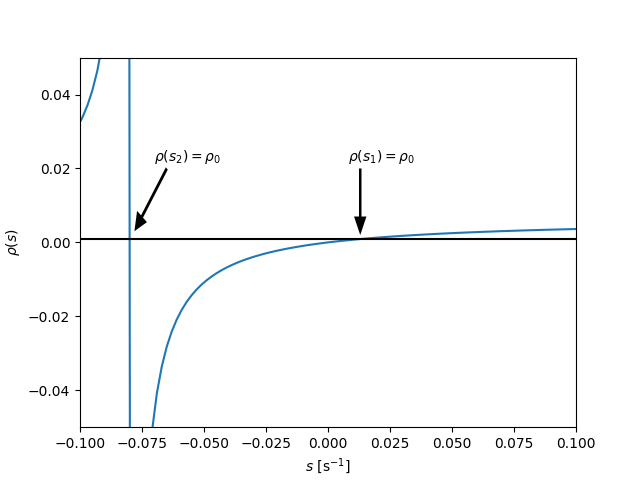
\includegraphics[scale=0.7] {figures/inhour_one_group.png}}\protect
\caption{\label{fig:inhour_one_group} \footnotesize{The inhour equation for one effective group of delayed neutrons. The horizontal black line shows a reactivity change $\rho_0$ of 0.001. The two solutions, at $s_1$ and $s_2$, are shown.}}
\end{figure}

From Fig. \ref{fig:inhour_one_group}, it is clear that a positive reactivity insertion will yield an increase in the neutron density. This increase will be a combination of the exponential with a positive $s_1$ and the exponential with a negative $s_2$. For a negative reactivity insertion, both roots are negative, leading to a decrease in the neutron density (governed by two exponentials with different time constants). Fig. \ref{fig:prompt_delayed_diff} shows the (numerical) solution to the point kinetics equations for one group of delayed neutrons (Eqs. \ref{eq:point_kinetics1_one_group} and \ref{eq:point_kinetics2_one_group} in terms of the relative increase in the neutron density after a positive reactivity increase of 0.001. In addition, the increse in the neutron density when considering \emph{only} prompt neutrons (i. e. the solution to Eq. \ref{eq:diffusion_eq_expanded3}). Clearly, the delayed neutrons have a dramatic effect on the behaviour of the reactor: when only including prompt neutrons we observe the swift exponential growth shown in the Exercise above.
\begin{figure}[ht!]
\protect \centering{
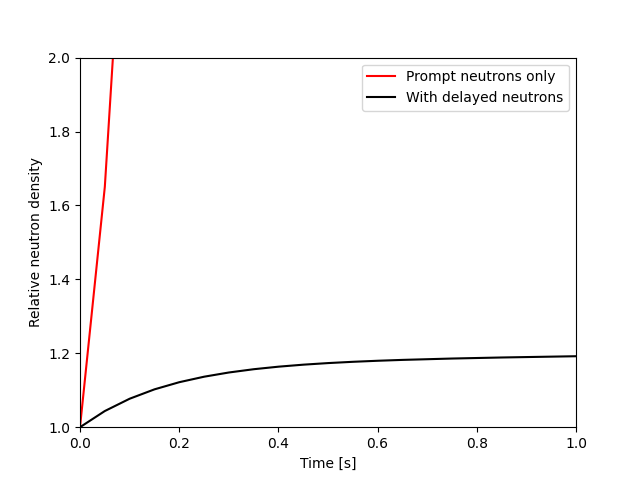
\includegraphics[scale=0.7] {figures/prompt_delayed_diff.png}}\protect
\caption{\label{fig:prompt_delayed_diff} \footnotesize{The relative change in the neutron density after a positive reactivity change of 0.001. The red line shows the solution when only including prompt neutrons (i. e. Eq. \ref{eq:diffusion_eq_expanded3} and the black line shows the solution when including one effective group of delayed neutrons (i. e. Eqs. \ref{eq:point_kinetics1_one_group} and \ref{eq:point_kinetics2_one_group}). The dramatic increase in reactor period when including delayed neutrons is visible.}}
\end{figure}

Finally, we can also illustrate the connection between the reactivity change, the precursor density and the neutron density. After all, Eqs. \ref{eq:point_kinetics1_one_group} and \ref{eq:point_kinetics2_one_group} are coupled differential equations so they must be solved simultaneously. Fig. \ref{fig:kinetics_solution_0001} shows a numerical solution to these equations, both for the neutron and the precursor density. One can see that the decay constant of the precursor $C$ is the same as the slower decay constant in the neutron density $n$, showing how delayed neutrons contribute to the overall time dependence of the neutron density in the core.
\begin{figure}[ht!]
\protect \centering{
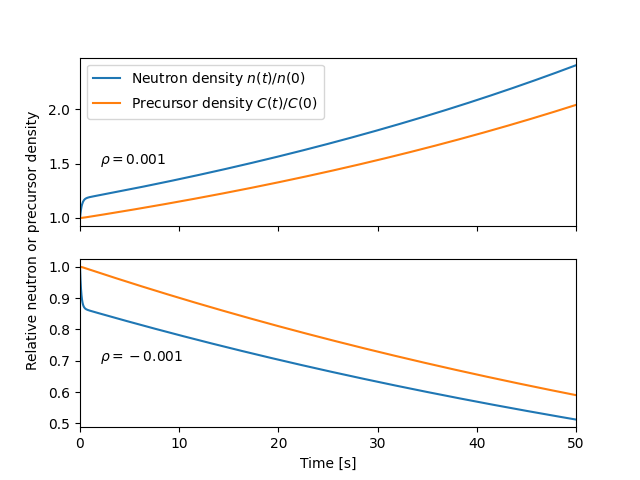
\includegraphics[scale=0.7] {figures/kinetics_solution_0001.png}}\protect
\caption{\label{fig:kinetics_solution_0001} \footnotesize{The relative change in the neutron and precursor density after a positive (top) and negative (bottom) reactivity change of $\pm0.001$. There is a rapid initial change in the neutron density (attributed to prompt neutrons), whereas the precursor density $C$ changes at a slower rate due to the associated longer half life. As a result, delayed neutrons emitted in the decay of precursors will contribute to the chain reaction at a much later stage, giving the slower exponential component in the neutron density.}}
\end{figure}

\subsubsection*{Six groups of delayed neutrons}
We may now extend the results from the previous section to the more realistic case of six groups of delayed neutrons. In fact, if we introduce all six groups into the calculations above, the results will be rather similar, with the exception that we now have a sum of seven exponentials instead of two in the final expressions for $n(t)$ and $C(t)$. For example, the time-dependence of the neutron population with six delayed-neutron groups is:
\begin{equation}
	n(t) = \sum_{i=1}^7 A_i \exp[s_i t],
	\label{eq:n_delayed_sum}
\end{equation}
This case is evidently more complex than the one-group treatment, but we can nonetheless gain some insight by looking at the inhour equation for six groups of delayed neutrons. In a similar manner, this will become
\begin{equation}
	\rho(s) = \frac{sl}{sl + 1} + \frac{1}{1 + sl}\sum_{i=1}^6 \frac{s\beta_i}{s+\lambda_i}.
\end{equation}
Using the data in Table \ref{tab:delayed_n} (remember that the decay constant is directly related to the half life) and $l = 10^{-4}$ seconds we may plot the six-group inhour equation, as shown in Fig. \ref{fig:inhour_six_group}. Clearly, there are seven roots to this equation, where only $s_1$ can be positive and the others are always negative. Again, the stable reactor period is given as $T = 1/s_1$. The asymptotic behaviour of the inhour equation appears at $s = -\lambda_1$, $s = -\lambda_2$, ..., $s = -\lambda_6$, $s = -1/l$.
\begin{figure}[ht!]
\protect \centering{
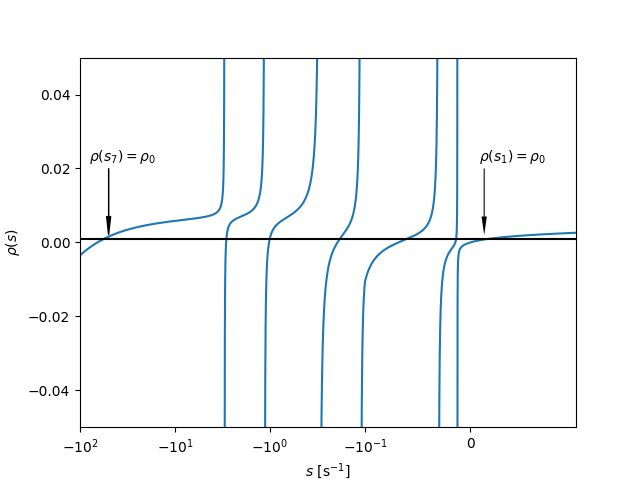
\includegraphics[scale=0.7] {figures/inhour_six_group.png}}\protect
\caption{\label{fig:inhour_six_group} \footnotesize{The inhour equation for six groups of delayed neutrons. The horizontal black line shows a reactivity change $\rho_0$ of 0.001. Two of the seven solutions, at $s_1$ and $s_7$, are shown. The horizontal axis is in a ``symmetrical logarithm'' scale.}}
\end{figure}

Although it is quite difficult to solve Eq. \ref{eq:n_delayed_sum} to get $n(t)$ for a certain reactivity change $\rho_0$. Nonetheless, the methodology we have used allows us to get a description of the time-behaviour of $n(t)$, which gives us some boundaries for safe reactor operation. In that context, we are finally interested in estimating the stable reactor period $T$ in a system with six groups of delayed neutrons. This is, as stated above, given by the inverse of $s_1$, which is the only positive root of $\rho(s) = \rho_0$. To get this, we resort to numerical tools for root finding. Fig. \ref{fig:reactor_period} shows the stable reactor period when including six groups of delayed neutrons as a function of the reactivity change $\rho_0$ given the approximate prompt-neutron lifetime in a thermal reactor: $l = 10^{-4}$ seconds. From this plot, we may directly read off the stable reactor period for a positive reactivity change of $\rho_0 = 0.001$ (corresponding to a change in $k$ from 1 to 1.001, as was investigated for the prompt system): $T \simeq 55$ seconds. This is a remarkable increase compared to the value of 0.1 seconds we obtained when not including delayed neutrons. That is, even though the delayed neutrons make up less than 1\% of the total neutron population, they are vital for controlled operation of a nuclear reactor! For comparison, Fig. \ref{fig:reactor_period} also includes the reactor period when only including prompt neutrons, as defined in Sec. \ref{sec:prompt_neutrons}. Clearly, the delayed neutrons increase the reactor period.
\begin{figure}[ht!]
\protect \centering{
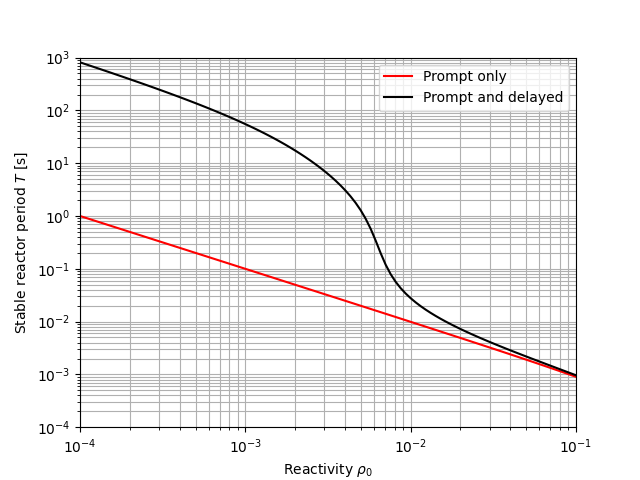
\includegraphics[scale=0.7] {figures/reactor_period_thermal.png}}\protect
\caption{\label{fig:reactor_period} \footnotesize{The reactor period $T$ as a function of the (positive) reactivity change $\rho_0$ in a thermal reactor characterised by a prompt neutron lifetime of $10^{-4}$ seconds. The two lines show the period when only including prompt neutrons and when also including six groups of delayed neutrons.}}
\end{figure}

We have now obtained a method to calculate the time behaviour of an operating nuclear reactor. We have seen that delayed neutrons introduce slower variations in the neutron population in the core, which in fact allow an operator to respond to various changes in the reactivity in the core. Of course, the description we have arrived at also allows us to understand how the system responds to reactivity changes \emph{not} controlled by the operator. Therefore, understanding the time behaviour of the system allows us to determine safety margins for reactor operation, and to construct a reactor that can operate safely. It is finally worth to discuss some concrete consequences of the results of this chapter.

\subsubsection{Concrete examples}
\subsubsection*{Reactor shutdown}
Even without discussing concrete measures used to control the reactivity in the core (such as control rods), the plot of the six-group inhour equation in Fig. \ref{fig:inhour_six_group} tells us something interesting about the shutdown of a nuclear reactor. To shut down a reactor, negative reactivity should be inserted (i. e. $\rho_0 < 0$). In such a case, all roots $s_{1-7}$ to the inhour equation are negative, meaning that the neutron population will go towards zero (which we want). The root with the highest value will be $s_1$, and as mentioned previously the asymptotic behaviour of the inhour equation occurs at $s = -\lambda_1$, $s = -\lambda_2$, ..., $s = -\lambda_6$, $s = -1/l$. This means that even if $\rho \rightarrow -\infty$, $s_1 \rightarrow -\lambda_1$. This characterises the longest time-dependence in the core, which is then given by a period of $1/\lambda_1$. Using the value for the half life of group 1 from Table \ref{tab:delayed_n}, calculating $\lambda_1$, $1/\lambda_1 \approx 80$ seconds. This will determine the fastest time scale on which the reactor can be shut off.

\subsubsection*{Prompt criticality}
Considering the point kinetics equation Eq. \ref{eq:point_kinetics1}, we see that the first term is negative for all $\rho < \beta$. That is, to make the system critical (i. e. $dn/dt = 0$), the delayed neutrons are needed to balance the equation. However, what would happen if $\rho = \beta$? Then the first term would become zero, and the other terms (the delayed neutrons) are not needed to make the system critical. That is, the system is critical on prompt neutrons alone --- we have reached a state called \emph{prompt criticality}. In such a case, we would again arrive at the situation where the reactor period becomes quite short. This is seen in Fig. \ref{fig:reactor_period}, where the reactor period in the system with delayed neutrons starts to approach the one in the prompt-neutron only system for $\rho_0 > \beta$ ($\beta = 0.0065$ in the system considered). Therefore, positive reactivity insertions are typically limited to $\rho_0 < \beta$. In fact, counting reactivity in units of $\beta$ is often done, where a reactivity change of $\beta$ is one \emph{dollar}. Some reactors are in fact able to operate in a pulsing mode, where the system is brought to a critical state after which reactivity is inserted (by removing control rods) to yield a rapid pulse of output power [https://www.youtube.com/watch?v=qCH3Yiyw3yc]. The reactivity increase will in such cases be balanced by a reactivity decrease provided by the temperature increase in the fuel [1].






%%%%%%%%%%FROM ERIK

\subsection{Subcritical multiplication}
When starting a nuclear reactor, the core is sub-critical with some margin, and the reactor does not produce any power. To start it, the reactor operator must remove control rods until the reactor reaches criticality. It is important here that the operator knows when criticality is reached, so that a safe doubling time is achieved. Since the reactor is at zero power, it is not possible to measure the doubling time by measuring the heat output. The key observable that can be measured at this point is the neutron flux. And as we have seen previously, the neutrons are tightly coupled to the multiplication in the system. The neutrons can originate from several different processes in a sub-critical system:

\begin{itemize}
\item Through spontaneous fission. The source is predominately U-235 in fresh fuel, with additions from Plutonium and Curium isotopes in used fuel. Each isotope has its own average neutron multiplicity for spontaneous fission, but typically around 2-3 neutrons are emitted per fission.

\item Through ($\alpha$, n) reactions. Heavy isotopes such as uranium and plutonium alpha decays, and when the alpha particle interacts with light elements such as oxygen, the alpha particle can be absorbed, with a neutron emission following. For reactors, the most common fuel is UO2, hence there is a lot of oxygen present. This reaction sends out a single neutron.

\item Through induced fission. Neutrons emitted by spontaneous processes can induce both fast and thermal fission in the sub-critical reactor, which creates further neutrons. 
\end{itemize}

If the rate of spontaneous fission neutrons and ($\alpha$, n) is $S$, then these will create an average $k \cdot S$ induced fission neutrons, which in turn creates $k^2 \cdot S$ neutrons e.t.c. Since the reactor is sub-critical, the total neutron emission rate $N$ is given by

\begin{equation} \label{eq:total_neutron}
N = S + k \cdot S + k^2 \cdot S + ... = \frac{S}{1-k} 
\end{equation}

Thus, the total neutron emission will depend both on the neutron source and the criticality, and more information is needed to be able to determine both parameters than only the total neutron count.  

Besides sub-critical cores, there are other times when sub-critical multiplication is of interest to measure. To give a few examples, when measuring nuclear material in bulk form to verify its properties, the multiplication provides information about the material composition, which can be used for example to verify enrichment. When nuclear fuel assemblies are stored outside of the reactor, they should never reach criticality, but each assembly in itself is a system where sub-critical multiplication happens. As a final example, in accelerator-driven systems, the reactor core has some margin to criticality, and an external accelerator system provides the neutrons to sustain the nuclear reaction. Equation \ref{eq:total_neutron} shows that near criticality, a relatively modest source is sufficient to create a much larger neutron flux due to multiplication. However, the core itself is always sub-critical, and the external source is required to sustain the fission chain reaction.

\subsubsection{1/M plots}

If the reactivity worth of a control rod is know, one method to determine the criticality is to measure the neutron flux, withdraw a control to add a know reactivity to the core, and measure again. This method is called the 1/M method. Such a procedure alters the neutron flux by changing the criticality, but the source term is not changed. Hence, only one parameter changes in equation \ref{eq:total_neutron}.

If $S$ is the number of source neutrons, a control rod is withdrawn to get a new $k = k_1$, and a new total neutron emission $N_1$ following equation \ref{eq:total_neutron}. This is illustrated in figure \ref{fig:1overm}.

\begin{figure} 
\centering
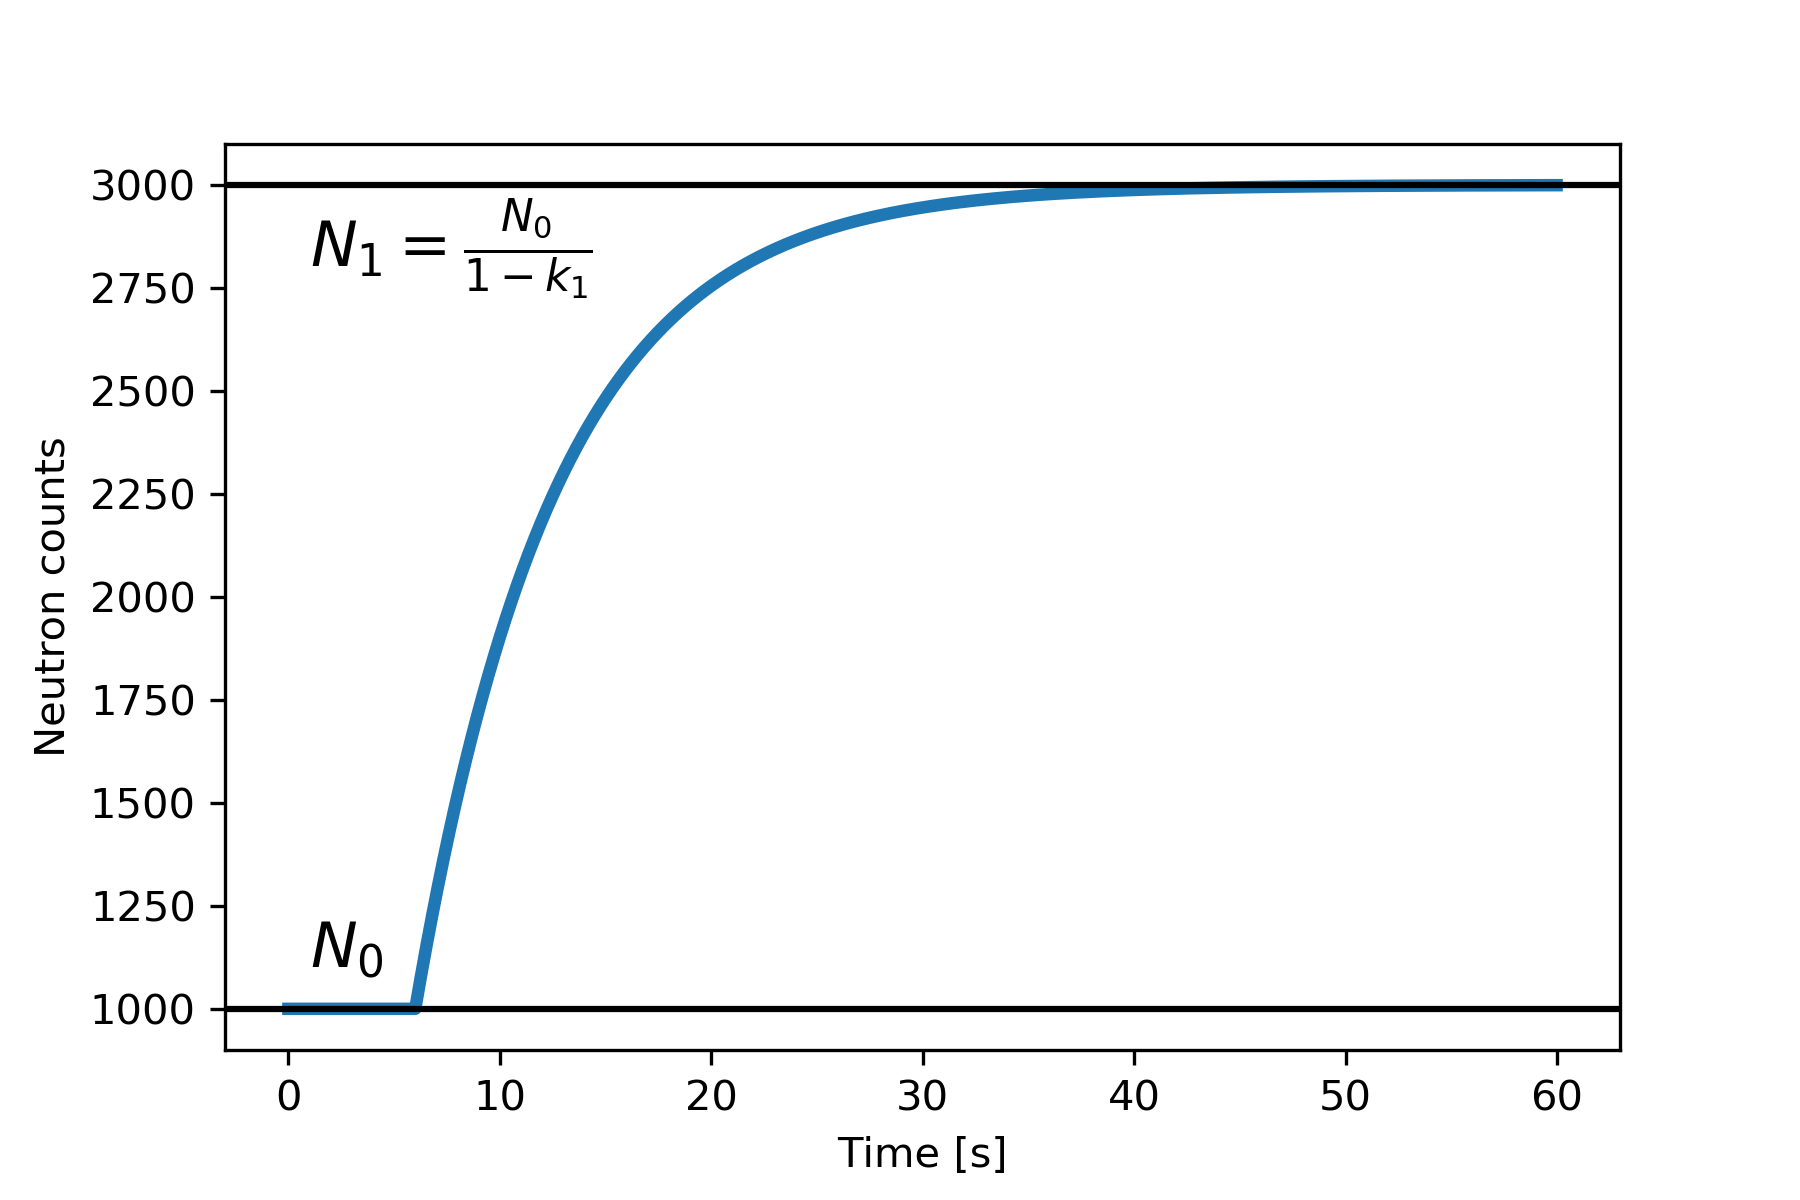
\includegraphics[width=0.8\textwidth]{figures/04-1overM.png}
\caption[Area Method]{\label{fig:1overm}
The effect on the neutron population when withdrawing control rods.}
\end{figure}

Now, the multiplication $M$ is defined from equation \ref{eq:total_neutron} as $M = 1/(1-k)$, and we then have:

\begin{equation} \label{eq:1overm}
\frac{S}{N} = \frac{1}{M} =  1-k
\end{equation}

Note that $1/M$ is linear in $k$. If we measure $1/M$ for a few different control rod positions, we can make a plot such as the one in figure \ref{fig:1overm_plot}

\begin{figure} 
\centering
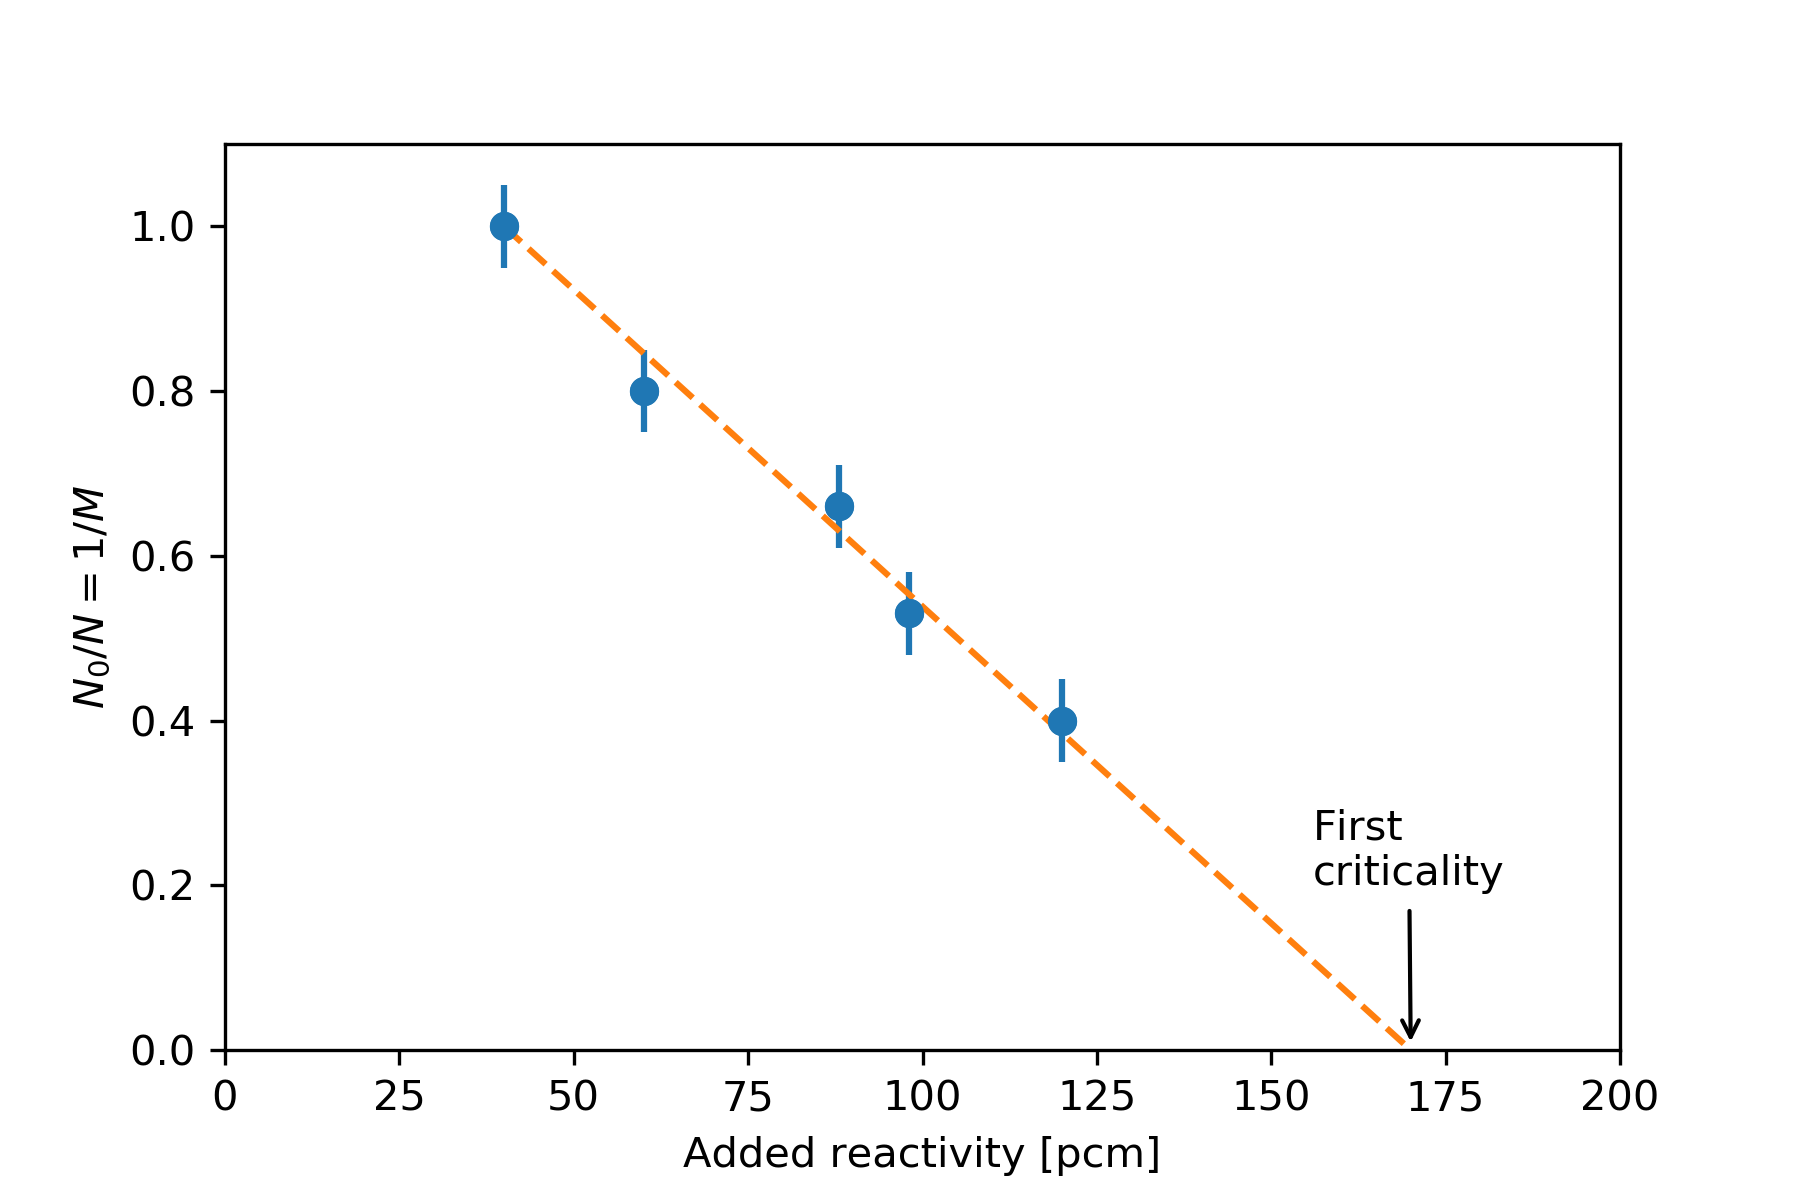
\includegraphics[width=0.8\textwidth]{figures/04-1overM_plot.png}
\caption[Area Method]{\label{fig:1overm_plot}
1/M plotted for a few control rod positions, and extrapolated first criticality.}
\end{figure}

By extrapolating the line formed by the $1/M$ measurements, it is possible to determine the criticality insertion necessary for first criticality. 

Note that in this method $S$ is not explicitly calculated, so we do not get a number for the neutron source. However, the $1/M$ method does not actually need $S$, only the relative change in neutron flux due to control rod withdrawal, which is measurable. Hence, even if we multiply equation \ref{eq:1overm} by some constant, this will not change where the equation is 0, i.e. where criticality is obtained.

\subsubsection{The Area method}

One method for determining the criticality is the so-called Area Method. In this method, a pulsed neutron source is used to interrogate the core. The neutron source will provide repeated, short bursts of additional source neutrons, which will induce fissions in the core. The detected neutron signal following one such pulse is shown in figure \ref{fig:area_method}

\begin{figure} 
\centering
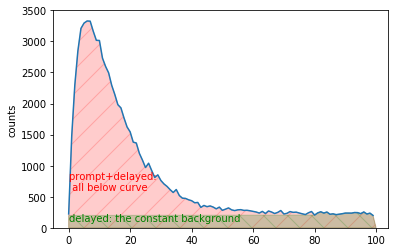
\includegraphics[width=0.8\textwidth]{figures/Area_method.png}
\caption[Area Method]{\label{fig:area_method}
The detected neutron signal when interrogating the core using a pulsed neutron source.}
\end{figure}

The number of prompt neutrons contained in the peak, $A_p$, is given by equation \ref{eq:prompt_neutron_area}, where $S$ is the source strength, and $\beta$ is the delayed neutron fraction.

\begin{equation} \label{eq:prompt_neutron_area}
A_p = \frac{S}{1-(1-\beta)k} 
\end{equation}

If the pulse neutron generator is kept active for sufficiently long, the delayed neutron fraction will reach an equilibrium, and the total number of  neutrons $A_d + A_d$, or the area in figure \ref{fig:area_method} is then given by equation \ref{eq:total_neutron_area}. Note that the delayed neutrons are typically emitted long after the pulse. However, for a constant pulsed source strength, the delayed neutrons from one pulse that occur after the measurement (after $t=100$ in figure \ref{fig:area_method}) is the same as the delayed neutrons from earlier pulses occurring within the measurement time. Hence, in equilibrium, the delayed fraction in figure \ref{fig:area_method} is actually the same as the total delayed neutron emission due to the pulse, if the measurement time is the same as the time between pulses. 

\begin{equation} \label{eq:total_neutron_area}
A_p + A_d = \frac{S}{1-k} 
\end{equation}

Thus, we can get the ratio of the total area to the prompt peak area as equation \ref{eq:neutron_area_ratio}. Note that the source strength $S$ cancels.

\begin{equation} \label{eq:neutron_area_ratio}
\frac{A_p + A_d}{A_p} = \frac{1-(1-\beta)k}{1-k} 
\end{equation}

And this equation simplifies to:

\begin{equation} \label{eq:neutron_area_ratio_simple}
\frac{A_p}{A_d} = - \frac{\rho}{\beta} 
\end{equation}

There is one more feature of interest in figure \ref{fig:area_method}, the exponential decay of the prompt neutrons, seen after the peak. Since it is exponentially decaying, its time evolution can be described by:

\begin{equation} \label{eq:area_decay}
\frac{dn(t)}{dt} = - \alpha \cdot n(t)
\end{equation} 

 $\alpha$ depends on the prompt neutron multiplication and mean neutron life time in the reactor. It can be shown that $\alpha$ can be expressed by:

\begin{equation} \label{eq:area_alpha}
\alpha = - \frac{\rho - \beta}{\Lambda}
\end{equation} 

Equation \ref{eq:area_alpha} can be rearranged into equation \ref{eq:area_lambda}, where the right hand side contains the ratio $\rho/\beta$ determined by equation \ref{eq:neutron_area_ratio_simple}, and alpha can be determined by fitting an exponential to the decay of figure \ref{fig:area_method}. If $\beta$ is also known, the neutron mean lifetime $\Lambda$ can be solved for.

\begin{equation} \label{eq:area_lambda}
\frac{\Lambda}{\beta} = \frac{1}{\alpha}(\frac{\rho}{\beta}-1)
\end{equation} 

\subsubsection{Rossi-alpha distributions}

For a sub-critical system with multiplication, the source neutrons (from spontaneous fissions and ($\alpha$,n) reactions) are created independently of each other, while induced fission neutrons follow a short while after a spontaneous neutron emission. Thus, by measuring the timing of the neutrons, it is possible to determine how many neutrons are uncorrelated, i.e. the source strength, and how many are correlated, i.e. the induced fission rate. One way to do this is to create a so-called Rossi-alpha distribution from the time interval between detected neutrons. 

To create a Rossi-alpha distribution, first a time-window must be defined, to determine the maximum time between neutrons that is of interest. This time window needs to be sufficiently long that all correlated neutrons occur within this time window, while still short enough that not all detected neutrons need to be compared to each other. Next, a histogram is created over the time difference between two detected neutrons, as long as the time difference is shorter than the time window. An example of how the Rossi-alpha times that are put in the histogram is constructed is shown in figure \ref{fig:neutron_timing}.

\begin{figure} 
\centering
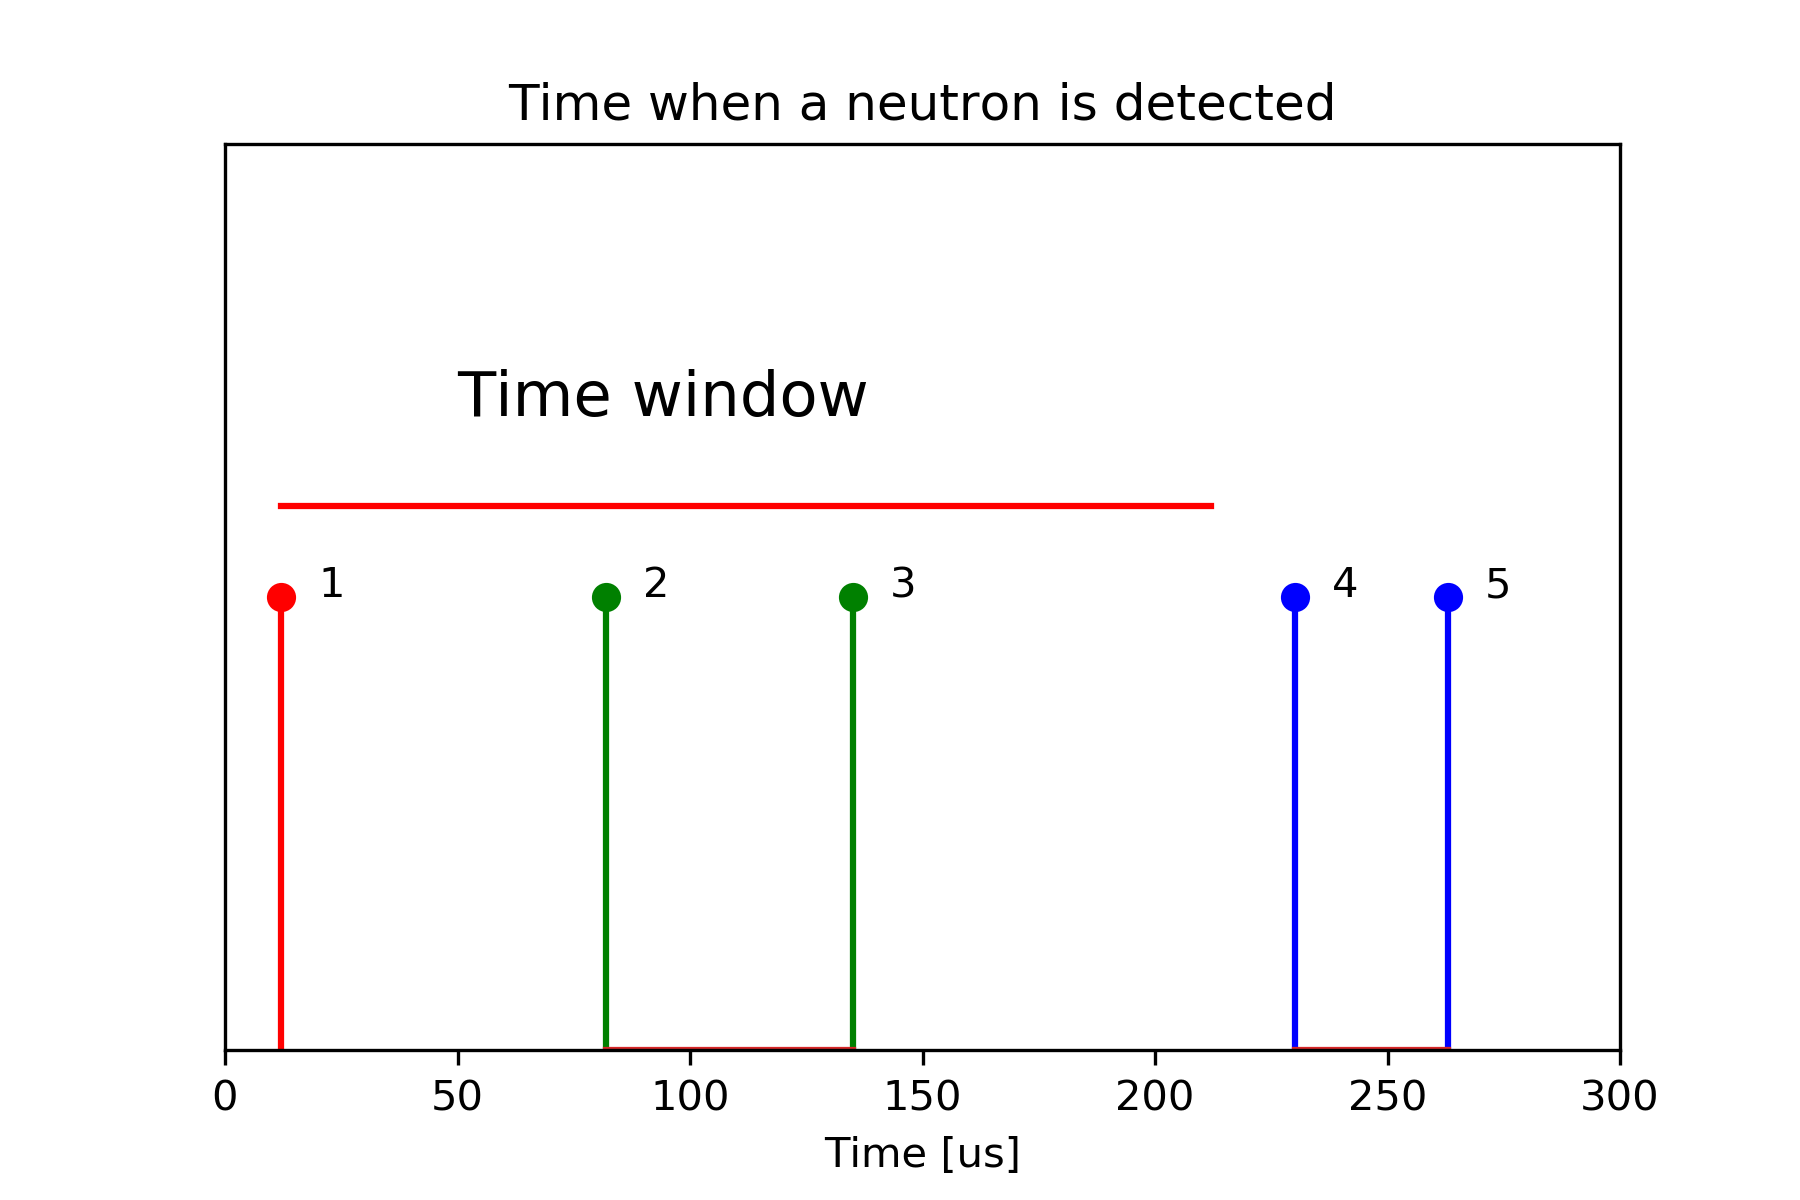
\includegraphics[width=0.8\textwidth]{figures/04-Neutron_timing.png}
\caption[Area Method]{\label{fig:neutron_timing}
Creating a Rossi-Alpha distribution from neutron detection timings. The neutron (1) is selected as the initial neutron, and neutrons (2-3) are then detected within the selected time window of 200 $\mu$s. The time differences between (1-2) and (1-3) are added to the histogram. Next, (2) is selected as the initial neutron, and the process is repeated for all neutrons within the time window after (2).}
\end{figure}

For uncorrelated neutrons, the time difference between the detection of the neutrons is random, hence each time difference is equally likely. Thus, uncorrelated neutrons will form a flat histogram. The correlated neutrons will however more likely have a short time difference, and in practice, will exponentially decay. For a system with multiplication, there are in fact two types of correlated neutrons. Neutrons originating fromt he same fission event, or from a subsequent induced fast fission, occur very close in time, and will thus correlate with a small time difference. For neutrons  in a fission chain where the neutrons thermalize before causing a fission, the neutrons are correlated but have longer times in between them. These two correlations define a fast and a slow die-away time, where the Rossi-alpha distribution can then be described by $H(t)$ in equation \ref{eq:rossi_alpha}. Here $A$ depends the spontaneous rate, $R_{fast}$ and $\tau_{fast}$ describes the correlated rate and decay time for the neutrons from the same event, and $R_{slow}$ and $\tau_{slow}$ describes the correlated rate and decay time for the neutrons from fission chains. Figure \ref{fig:rossi_alpha_plot} shows an example Rossi-alpha plot.  

\begin{equation} \label{eq:rossi_alpha}
H(t) = A + R_{fast} \cdot e^{-t/\tau_{fast}} + R_{slow} \cdot e^{-t/\tau_{slow}}
\end{equation} 

\begin{figure} 
\centering
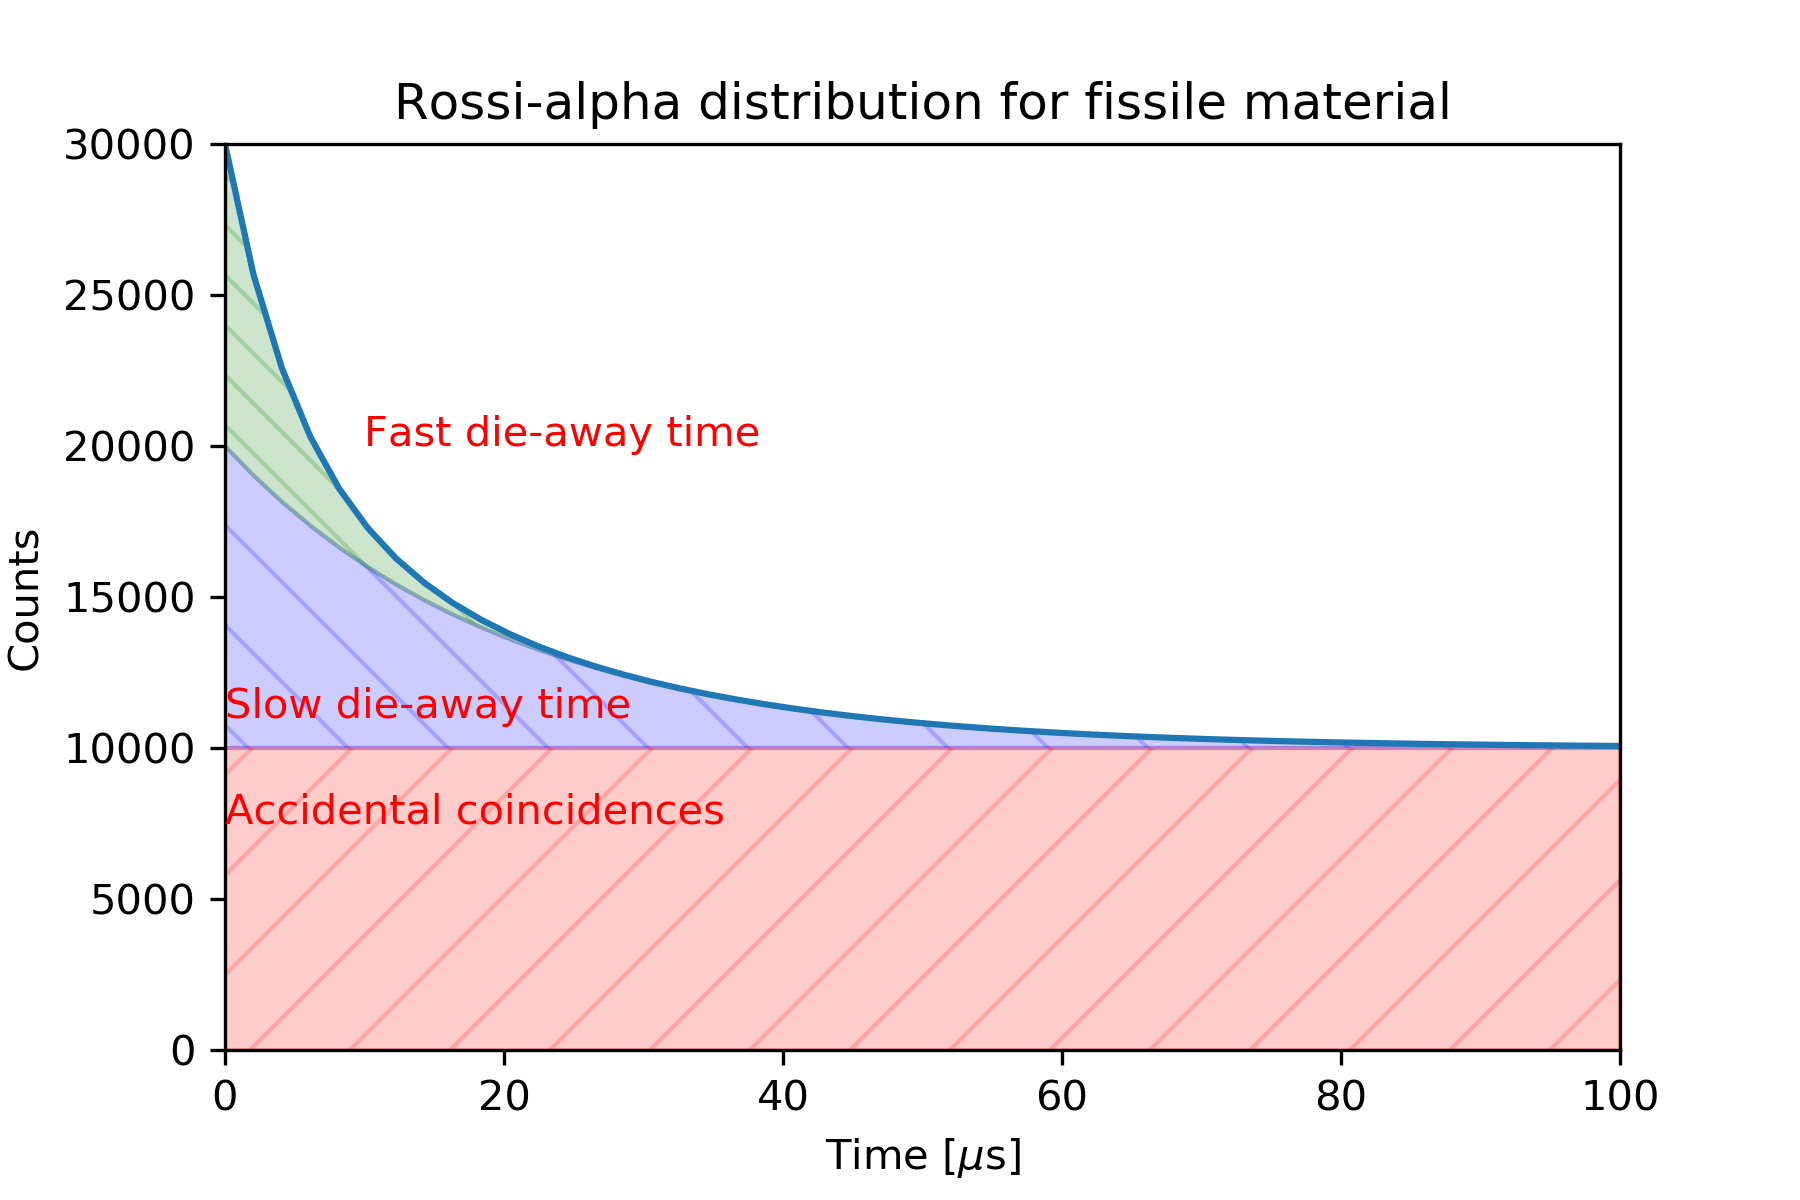
\includegraphics[width=0.8\textwidth]{figures/04-Rossi_alpha_slow_fast.png}
\caption[Area Method]{\label{fig:rossi_alpha_plot}
A Rossi-Alpha plot for a system with multiplication. The fast component is due to neutrons originating in the same fission event (or in a subsequent fast fission), the slow component is due to fission chains.}
\end{figure}

By investigating the slow die-away time, information is gained on the multiplication of the material. However, the fast component depends mainly on the properties of the source, and some effort is required to separate these two components. 

In the Rossi-Alpha distribution, every neutron is essentially considered to be a starting neutron, much as the source in the area method, and the subsequent induced fission neutrons behaves just as in the area method, with the same exponential decay. Hence, the exponential decay of the slow component can approximately be described using equation \ref{eq:area_decay} and \ref{eq:area_alpha}. Note however that only neutron from spontaneous fissions can act as a measurable starting signal, since they may emit enough neutrons to both be detected and to induce fission. Neutrons from ($\alpha$,n) reactions are always uncorrelated, since they are single neutrons. If such neutrons are detected, they cannot have induced fission, and if they induced fission, they are absorbed and cannot be detected. 

\subsection{Feedbacks}

In the previous lectures, we used the four-factor formula to calculate the criticality $k$, and the reactivity $\rho$. However, to understand the behaviour of the reactor, it is of interest to investigate how these parameters change as a function of other reactor parameters, such as fuel or coolant temperature, or reactor power. When the reactor is producing power, changes in the criticality (due to for example control rod movement) will change the power, which changes the temperatures, which in turn affect factors in the four-factor formula, and thus affect the criticality. This feedback defines the dynamics of the reactor.

One convenient approximation that can be used when $k$ does not significantly differ from 1 (which is the usual case when the reactor is running) is:

\begin{equation} \label{eq:dk_approx}
d\rho = dk^2/2 \approx dk/k = d(ln k)
\end{equation} 

If we apply this approximation to the four-factor formula, the logarithm results in that the multiplied factors are added, which separates the factors.

\begin{equation} \label{eq:dk_dk}
\frac{dk}{k} = \frac{d\epsilon}{\epsilon} + \frac{dp}{p} + \frac{df}{f} + \frac{d\eta}{\eta}
\end{equation} 

For light water reactors, using water as both moderator and coolant, the temperature feedbacks are dominating, and we will look at those in more depth.

\subsubsection{Fuel temperature coefficient}
Out of the factors in the four factor formula, the resonance escape probability $p$ is the one most strongly affected by the temperature. As described in previous chapters, this is due to the Doppler broadening of the resonance peaks, which means that neutrons are more likely to be captured in U-238 as the temperature increase, which lowers the reactivity. To describe the fuel temperature feedback, we introduce a fuel temperature coefficient $\alpha_f$ that relates the changes in fuel temperature $T_f$: to changes in the reactivity:

\begin{equation} \label{eq:alpha_f}
\alpha_f = \frac{1}{k}\frac{\partial k }{\partial T_f} \approx \frac{1}{p}\frac{\partial p}{\partial T_f}
\end{equation} 

And using the resonance integral to calculate the probability of resonance capture $I$, $\alpha_f$ can be calculated as:

\begin{equation} \label{eq:alpha_f_I}
\alpha_f = - \ln \left(\frac{1}{p}\right)\frac{1}{I}\frac{\partial I}{\partial T_f}
\end{equation} 

For a reactor at full power, we can approximate $\alpha_f$ to be constant over a moderate temperature change, and the change in reactivity $\Delta \rho$ due to a temperature change of $\Delta T_f$ is simply

\begin{equation} \label{eq:delta_alpha_f}
\Delta \rho = \alpha_f \Delta T_f
\end{equation} 

\subsubsection{Moderator temperature coefficient}
For a liquid moderator, when the moderator temperature increases, its density decreases, which decreases the moderation of the neutrons. Consequently, resonance capture increases since the neutrons have on average more energy, and the thermal utilization factor $f$ also increases, since absorption in the moderator decreases. If $\beta_m$ is the volumetric coefficient of thermal expansion at constant pressure for the moderator, it can be shown that the moderator temperature coefficient can be approximated as:

\begin{equation} \label{eq:delta_alpha_m}
\alpha_m = -\beta_m [\ln(1/p) - (1-f)]
\end{equation}

Note that in equation \ref{eq:delta_alpha_m}, the contribution due to $p$ and $f$ have opposite signs. For a light water reactor, $p$ is the largest contributor to $\alpha_m$ for all normal operations, thus $\alpha_m$ is  negative. For solid-moderated reactors, such as the graphite moderated reactors in Chernobyl, the thermal expansion of the moderator is less pronounced, and the factor $f$ may dominate $\alpha_m$, which then becomes positive at certain temperatures. For such reactors, an increase in power leads to an increase in temperature, which increases $f$ and thus $\alpha_m$, which further increases the power, which allows a runaway power increase. 

For boiling water reactors, additional heat in the reactor will result in the production of more steam, which take up more space than the water in the core. As a consequence, the moderator density changes significantly with the power, and the moderator temperature feedback is high for such reactors. In a pressurized water reactor, extra heat will only decrease the moderator density slightly, and it is instead the fuel temperature feedback which provides the largest change with temperature. 

\subsubsection{Excess reactivity margins}
The previous sections have shown that for light water reactors, $\alpha_f$ and $\alpha_m$ are negative, and will suppress a change in power. Thus, when starting a reactor from a room-temperature state, controllable poisons (control rods, soluble boron or both) must continuously be withdrawn to increase the power, to compensate for the effect of the feedbacks. To further illustrate this effect, parameters called the power defect and the temperature defect can be introduced, together with a parameter called shutdown margin.

The shutdown margin is the reactivity difference between a core that has all control rods inserted (and is at maximum boron concentration for a pressurized water reactor), and a critical, cold core. Thus, the shutdown margin is an excess negative reactivity available to ensure that there is always sufficient controllable poisons to shut down the reactor, regardless of how it operates. 

The temperature defect is defined as the reactivity insertion needed bring the core from room-temperature ($T_room$) to near operating temperature ($T_hot$), while still producing little power. Since the feedbacks in general changes with temperature, the power defect $D_p$ can be written:

\begin{equation} \label{eq:D_t}
D_t = \int_{T_{room}}^{T_{hot}}\alpha_f(T) + \int_{T_{room}}^{T_{hot}}\alpha_m(T)dT
\end{equation}

Note that the reactor is usually brought to the hot temperature rather slowly, hence the moderator and fuel temperature will be essentially the same during the entire process, and the two integrals can be merged.

The power defect is defined as the reactivity insertion required to bring the core from a hot, zero-power state to a power-producing state. In this case, the fuel and moderator temperate will be different throughout the process, and have different operating temperatures $T_f$ and $T_m$.

\begin{equation} \label{eq:D_p}
D_p = \int_{T_{hot}}^{T_f}\alpha_f(T) + \int_{T_{hot}}^{T_m}\alpha_m(T)dT
\end{equation}

In addition to these three margins and defects, the consumption of U235 (and build-up of plutonium) also affects the reactor core. As fissile mass is depleted over time, the thermal fission factor $\eta$ decreases, and to maintain criticality more controllable poisons need to be removed. Hence, to operate the reactor for extended periods of time, additional criticality margin is needed, as compared to just the start-up process.

In total, the shutdown margin, temperature and power defect, and fuel burnup determines how much controllable reactor poisons are needed to operate the core. On one hand, the more controllable poisons are required, the easier it is to control the reactor, since large changes in poison inventory is required to make small changes in the reactor power. On the other hand, using too much controllable poisons is costly and can be complex to design, which may reduce reliability, and thus affect safety. When designing the reactor, these two factors must be balanced.


\subsection{Depletion: evolution of fuel}

During the operation of a nuclear reactor the nuclear fuel evolves. This evolution has some technological reasons (corrosion, swelling of the fuel pellets due to gaseous fission products, radiation damage), and reactor physics reasons. In this course we are going to focus only on the reactor physics aspects of this evolution. From our previous studies we already know that the processes leading to a change in the nuclide inventory of the fuel are the following:

\begin{itemize}
\item Due to fission events the amount fissile nuclei decreases. Thus the reactivity of the fuel decreases.
\item Due to fission event fission products appear in the fuel with medium mass number. Some of these nuclides have high absorption cross sections (they are considered to be \textit{reactor poison}.
\item Due to neutron capture of uranium nuclei transuranic elements are created, some of these nuclei are fissile.
\end{itemize}

Altogether these processes leading to the evolution of fuel are called burnup or depletion. When the fuel depletion reaches a level that the core cannot be critical anymore the fuel elements are replaced with fresh fuel. Due to safety reasons the core load is designed so, that when the fuel is fully depleted its amortization due to technological reasons still does not present any risk.

\subsubsection{Depletion chains}

As we saw before there are several neutron collision reactions (eg. fission, capture, (n,\textit{i}n) reactions), and several decay reactions which will transform a nuclide into an other nuclide. Similarly, as we saw before for decay series (Fig. \ref{fig:decaychain}, we can develop depletion chains, however these are fairly complex if every possible reaction is taken into account. The top of Fig. \ref{fig:depletionchain} shows all the (n,$\gamma$) and (n,2n) reaction, and all alpha and beta decay paths for when starting to irradiate U238, whereas the lower figure shows some of the most important paths for the uranium depletion chain.

\begin{figure}[ht!]
\protect \centering{
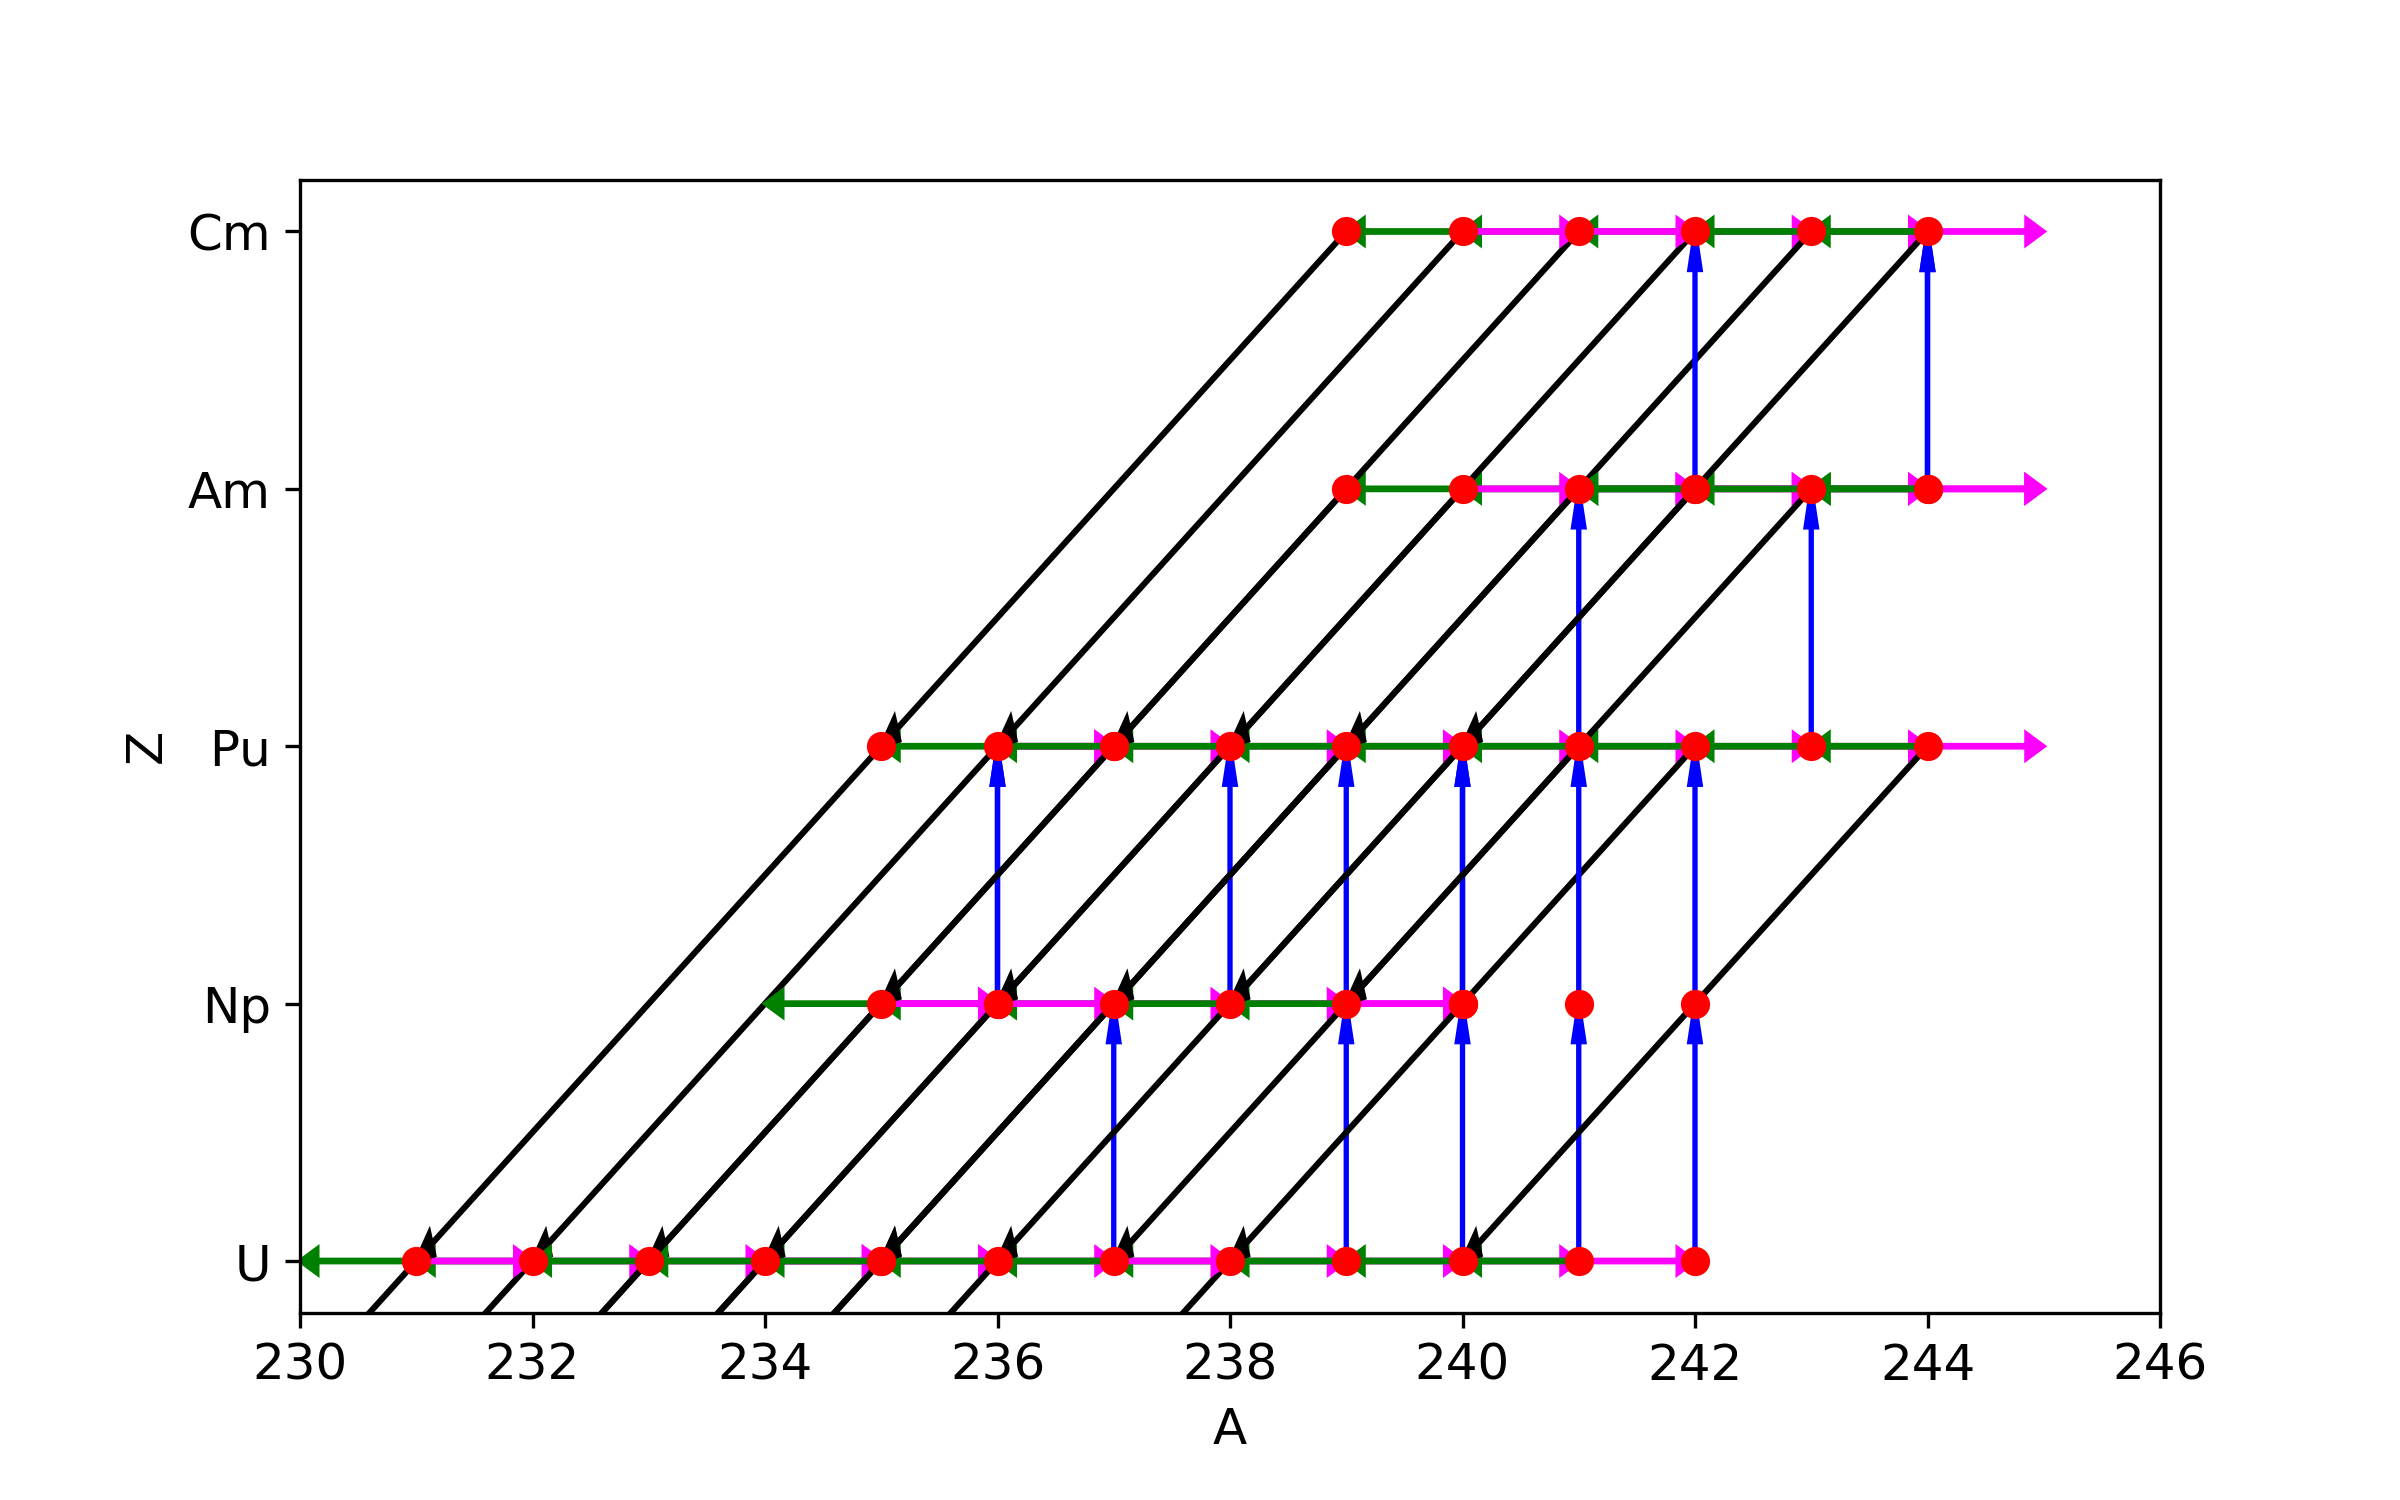
\includegraphics[scale=0.44] {figures/04-chaincomplete.png}
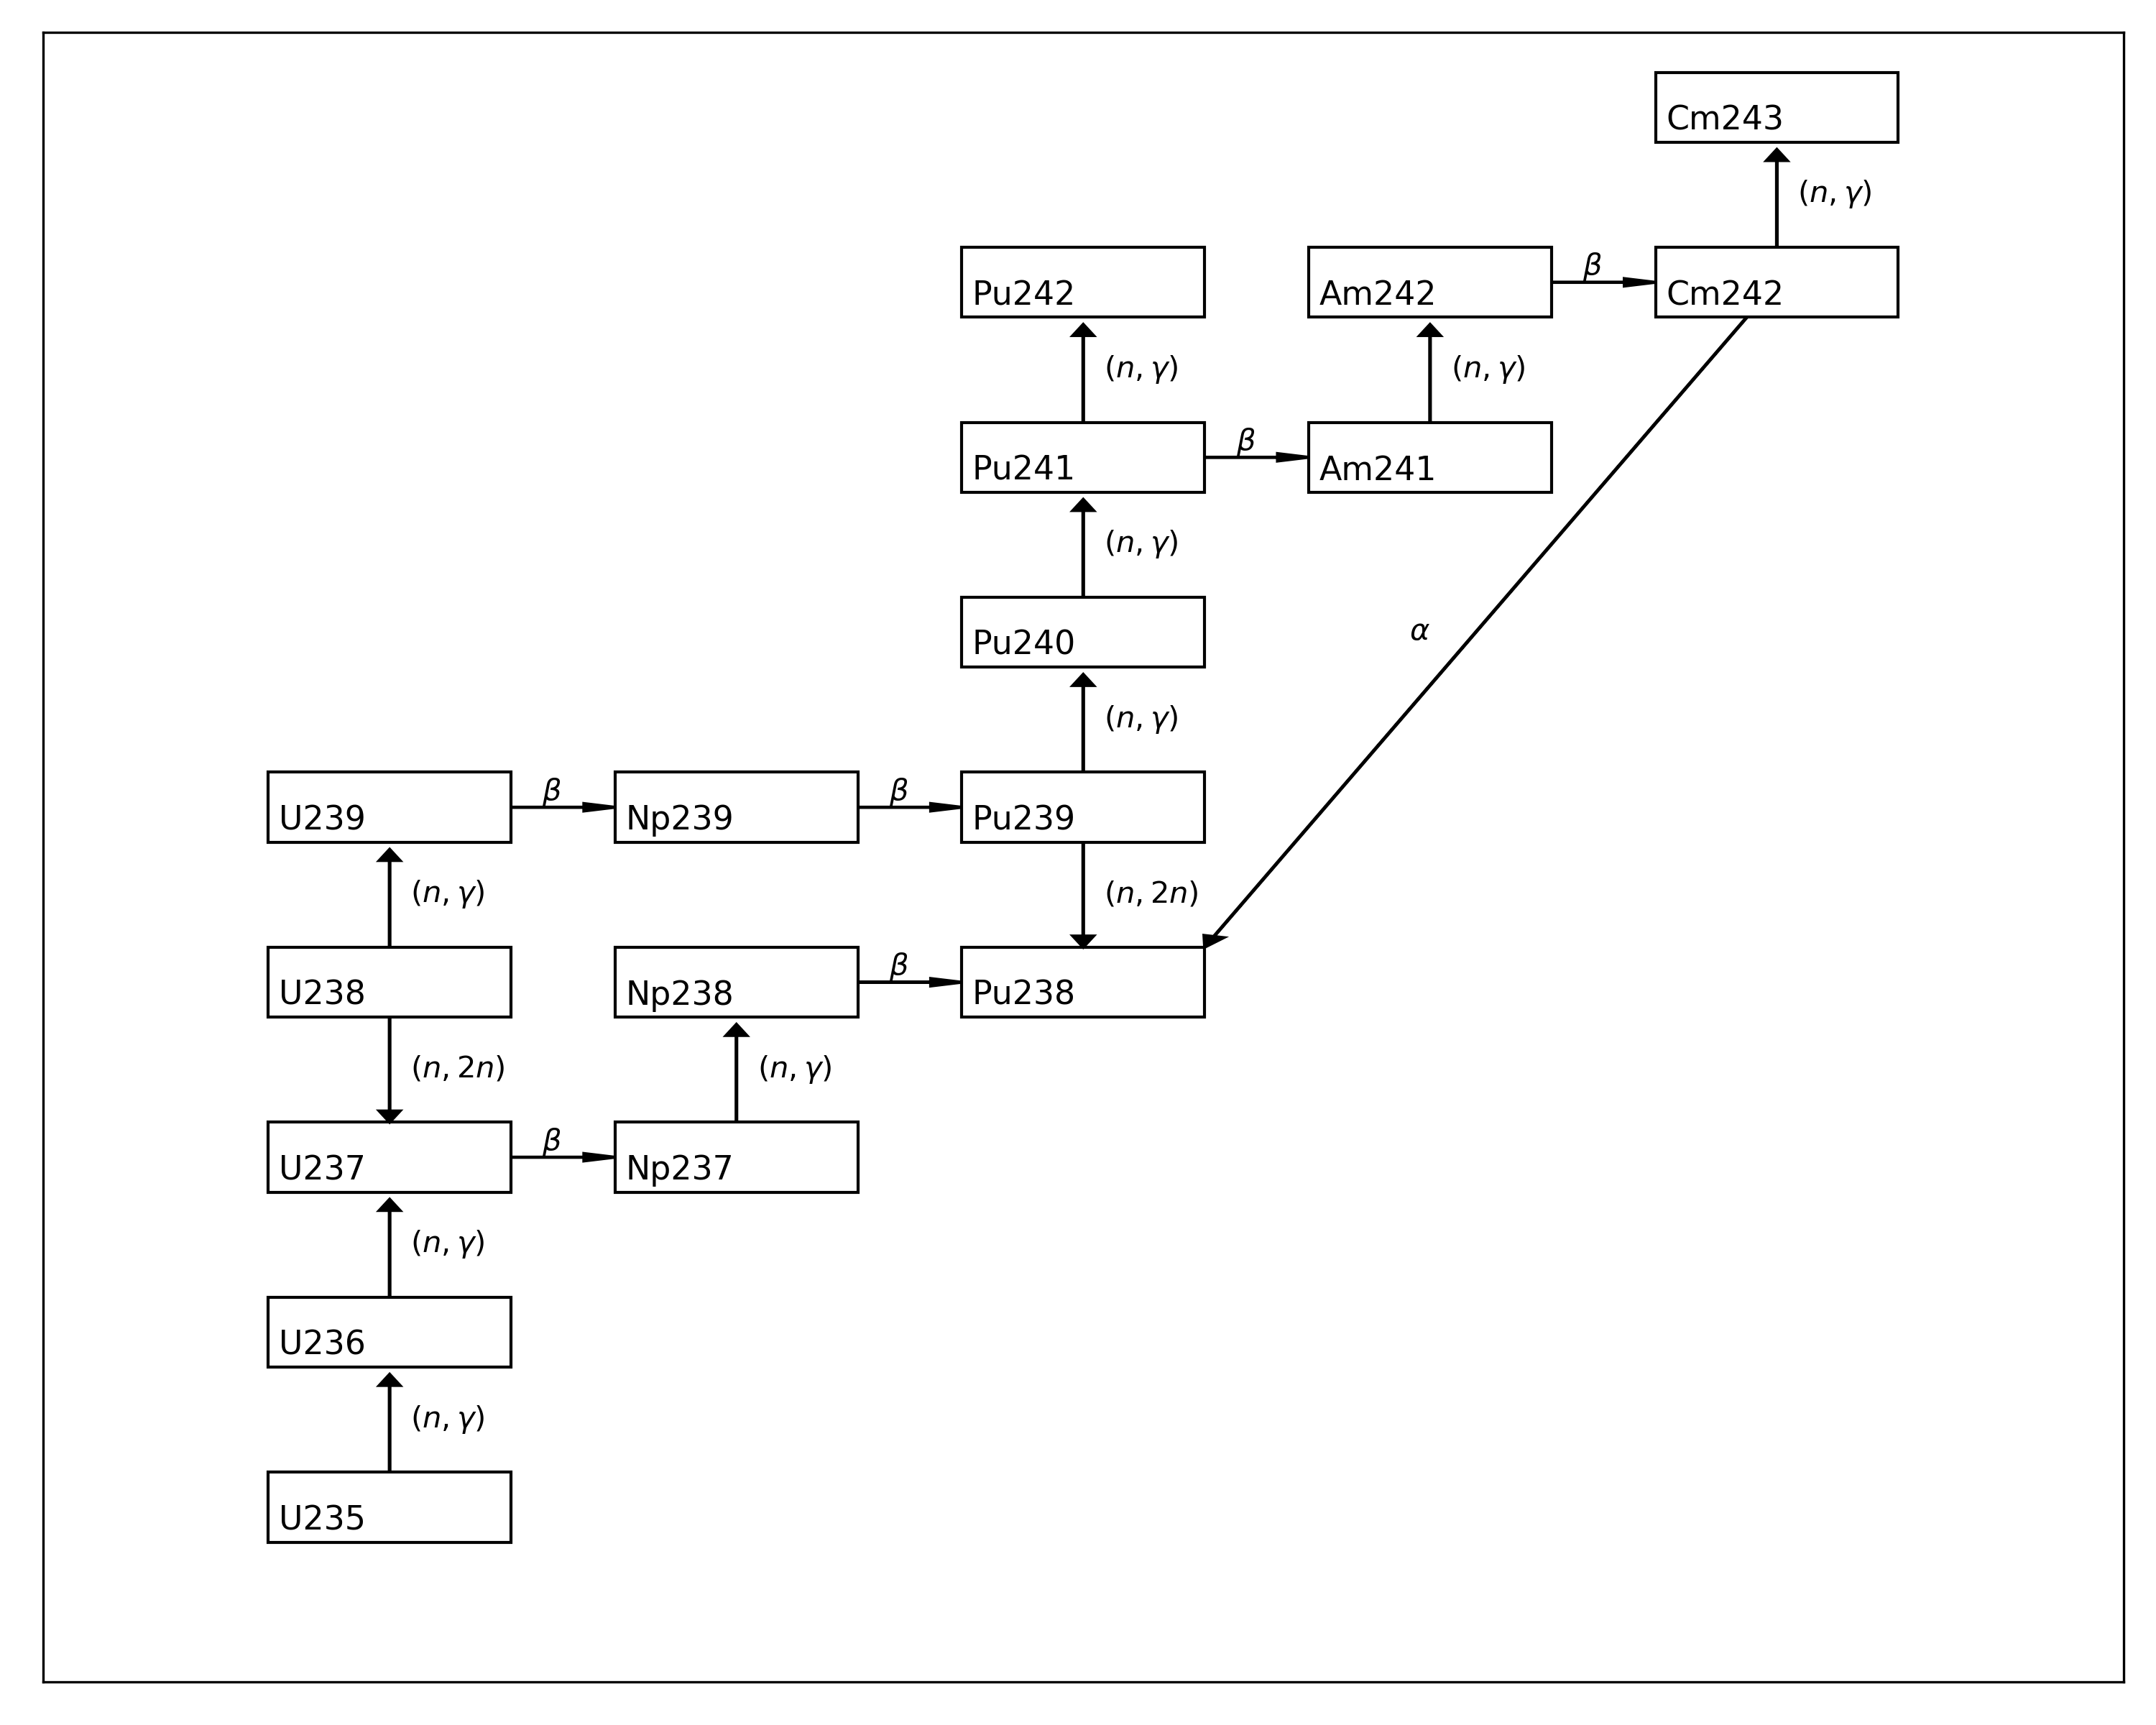
\includegraphics[scale=0.44] {figures/04-uranchain.png}}\protect
\caption{\label{fig:depletionchain} \footnotesize{Illustration of depletion chains.}}
\end{figure}

If we wanted to  make a very accurate analysis of the evolution of fuel under irradiation we should consider every possible scenario. How ever for practical applications we can simplify depletion chains. For example we can neglect the decay of uranium isotopes (and the neutron reactions on the daughters of these isotopes) due to the long half-lives. That said, we can consider different depletion chains for uranium fueled and thorium fueled reactors. (In thorium fuel reactors the Th232 nuclide is first converted into fissile U233, however they do not have yet a widespread use so in the following we do not discuss this).

\subsubsection{Batemen-equations}

In the following we will write up a rather general equation describing the depletion. However, first we will use some simple examples to review the basic concepts.

\subsubsection*{One nuclide with source and decay}

Now let's consider an example where we are interested in the time evolution of a  radioactive nuclide $N$ which is constantly created (for example from a neutron reaction for which the cross section is given by $\Sigma$ on a parent nuclide), and for which $N(t=0)=0$. We can consider that we have a lot of parent nuclei, therefore the change in its number is negligible (therefore the production rate is constant) This example is a very fair model for cases when a small target (for example a foil) is being irradiated, but it could be applicable for a fission product.

The change of amount (or density) of the nuclide $N$:

\begin{equation}
\frac{N}{dt}=-\lambda N + \underbrace{\Sigma\phi}_{\text{production rate}}
\end{equation}

\begin{equation}
N(t)=\frac{\Sigma\phi}{\lambda}[1-exp(-\lambda t)] \quad \Rightarrow \quad A(t)=\Sigma\phi[1-exp(-\lambda t)]
\end{equation}

\noindent where we can define the saturation activity (or saturation concentration) as $t\rightarrow \infty$:

\begin{equation}
A(t\rightarrow \infty)=A_s=\Sigma\phi
\end{equation}

\noindent We see that infinity the activity and the concentration would saturate at a constant level (if the parent nuclide is not lost). How quickly we reach this saturation level depends on the half-live of the nuclide (the longer lived the nuclide is the longer it takes to reach saturation). If the irradiation takes place only for a finite time $t_{irr}$ after which the material is left to "cool", then the new differential equation to describe the change is simply

\begin{equation}
\frac{N^{after}}{dt}=-\lambda N^{after}
\end{equation}

\noindent where "after" refers to "after irradiation". The initial condition of this differential equation is $N^{after}(0)=N(t_{irr}$. The solution is simply the exponential decay:

\begin{equation}
A(t_{cool}>t_{irr}=\Sigma\Phi[1-exp(-\lambda t_{irr})]\cdot exp(-\lambda t_{cool})
\end{equation}


\begin{figure}[ht!]
\protect \centering{
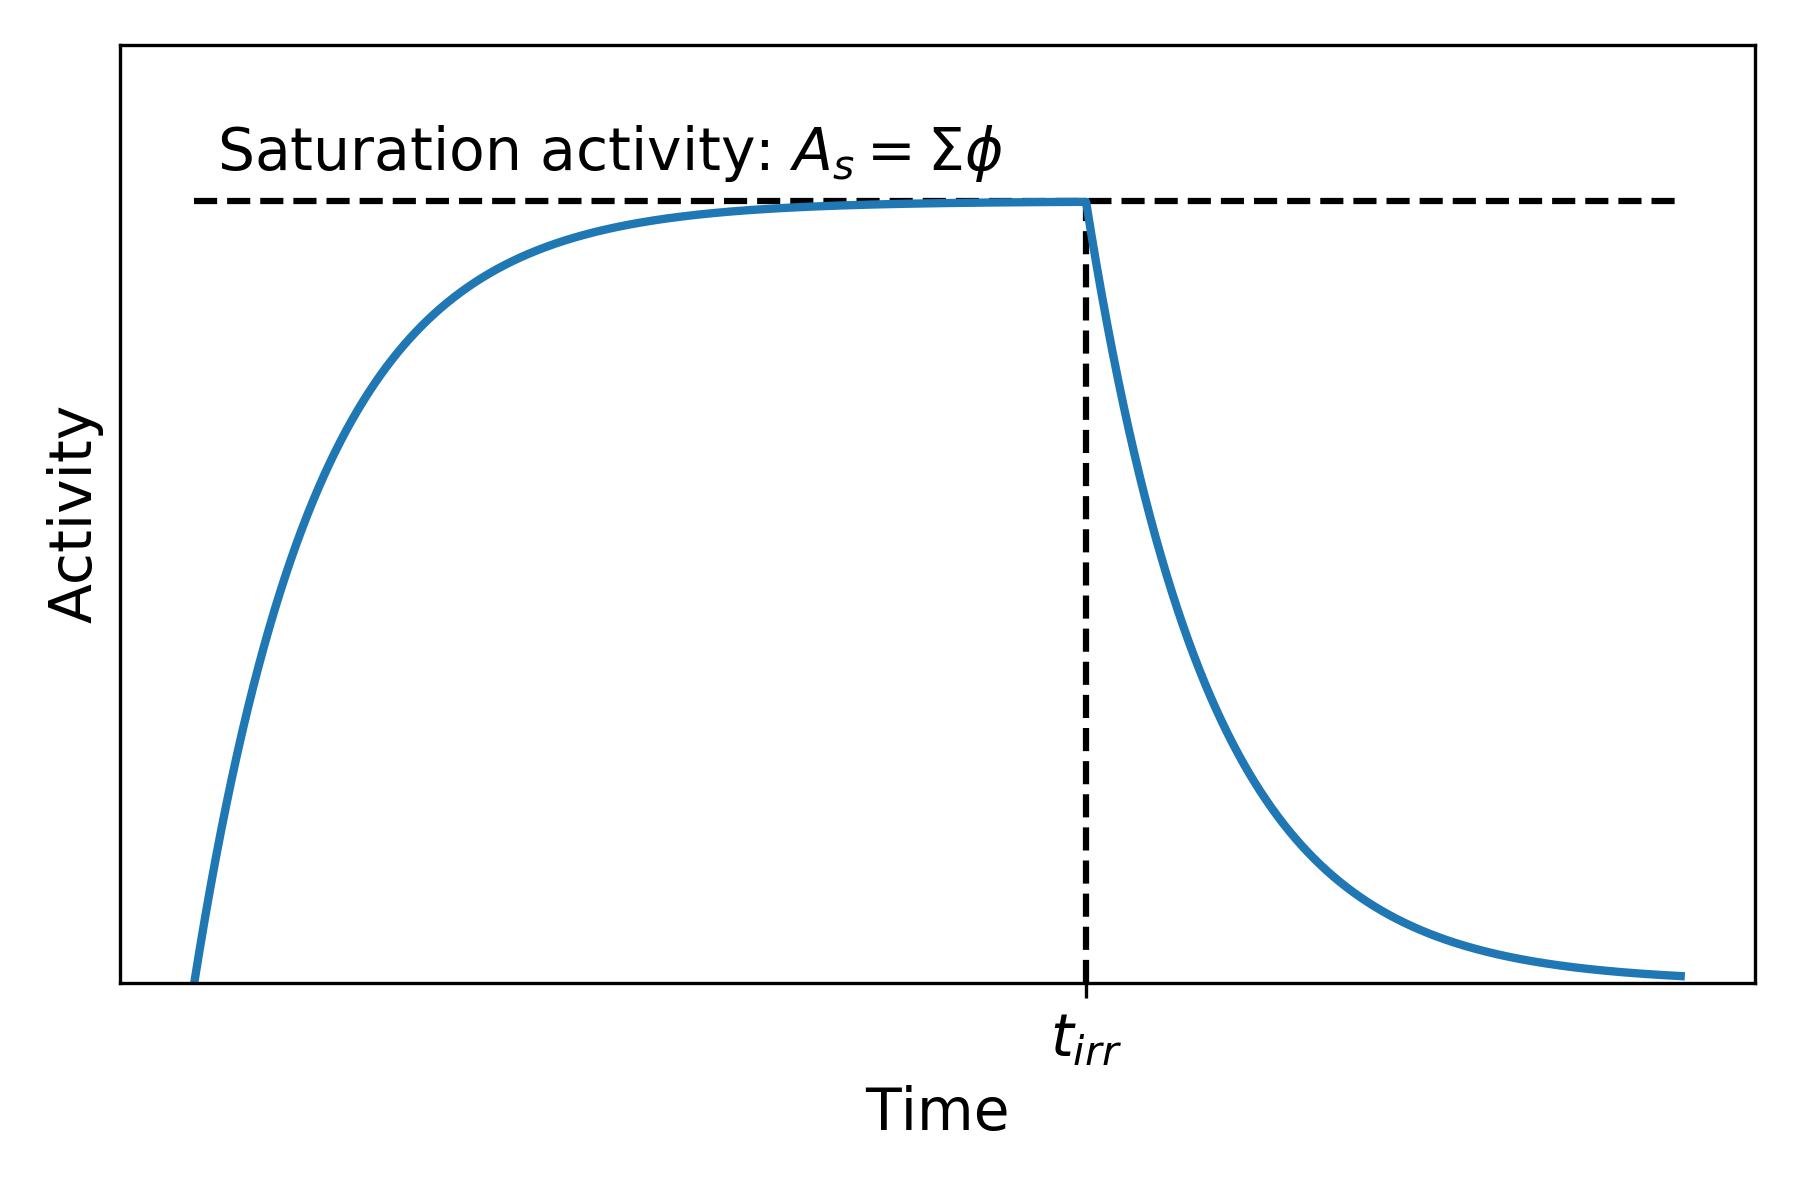
\includegraphics[scale=0.44] {figures/04-saturation_activity.png}
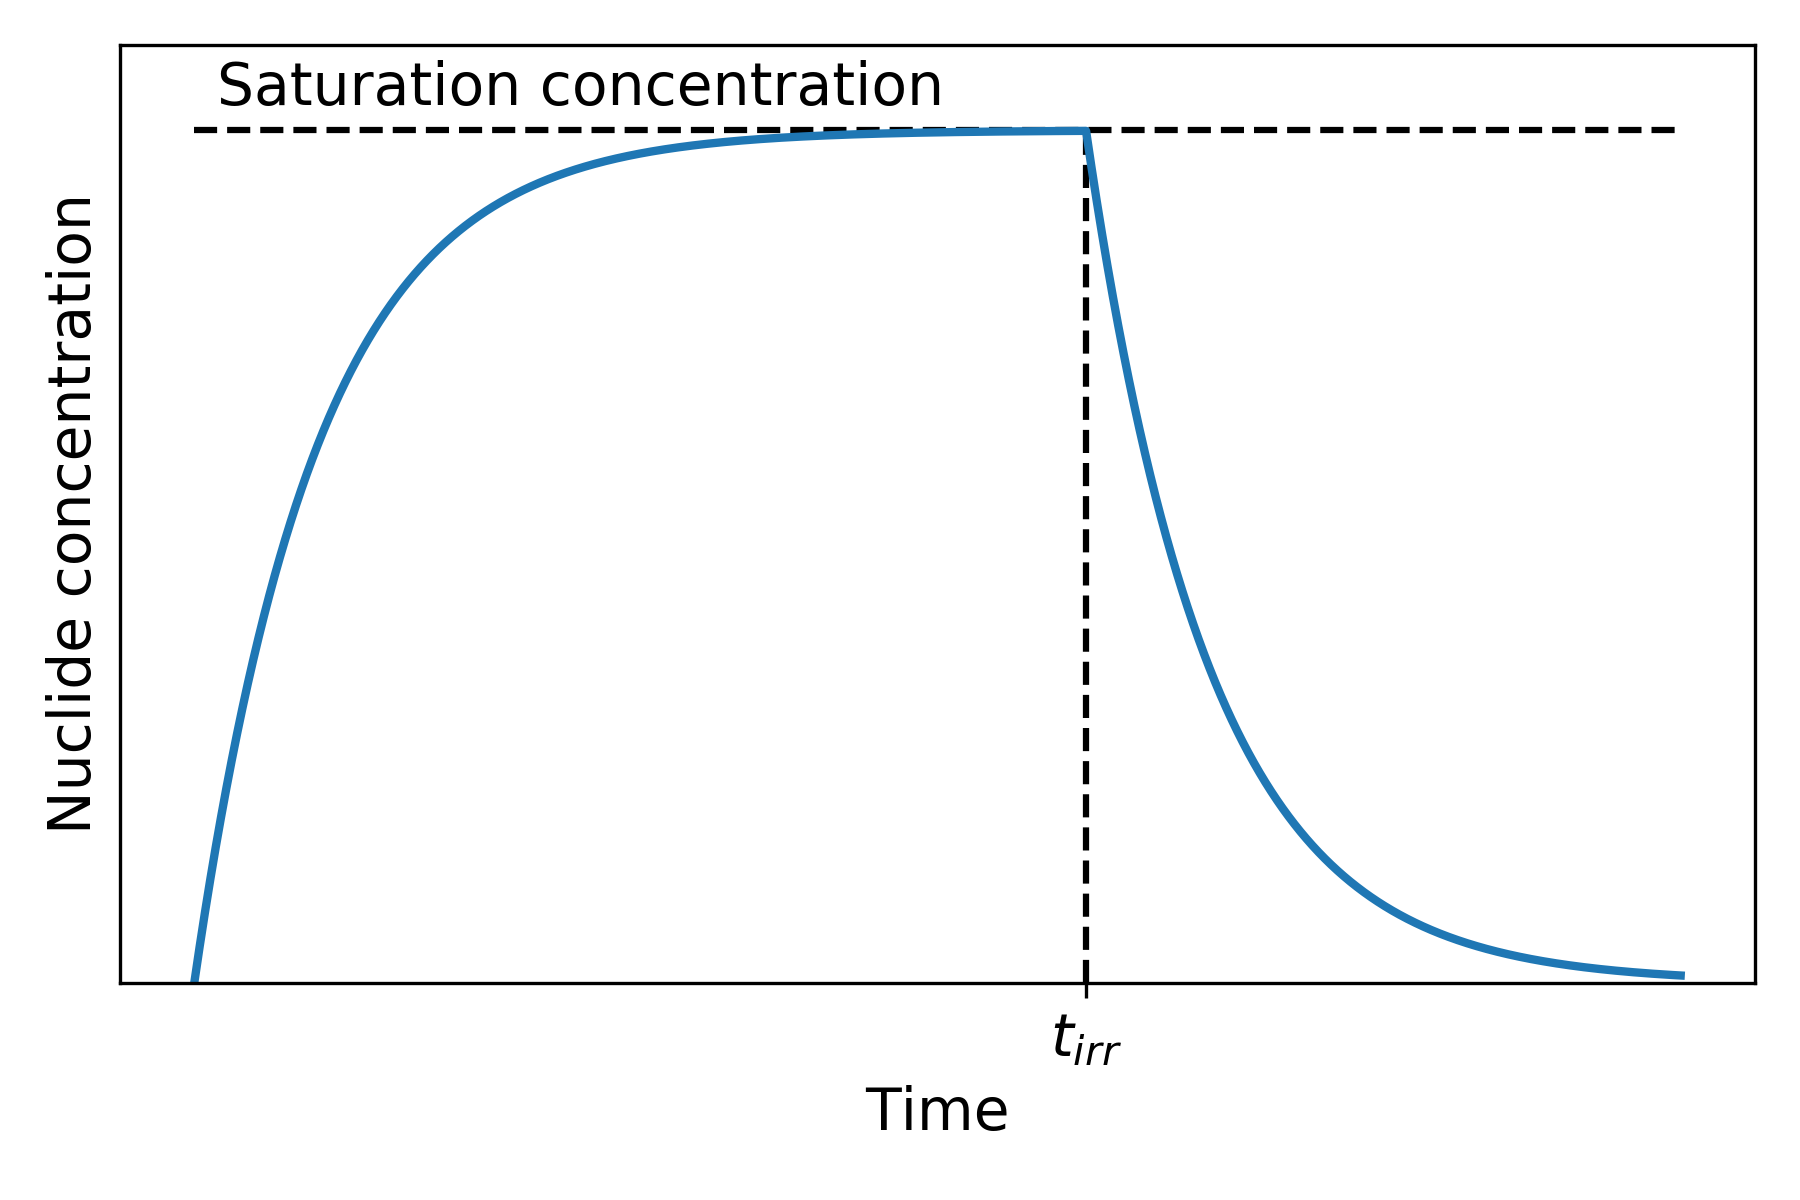
\includegraphics[scale=0.44] {figures/04-saturation_concentration.png}}\protect
\caption{\label{fig:irradiationconc} \footnotesize{Change of nuclide concentration during and after irradiation.}}
\end{figure}

Fig. \ref{fig:irradiationconc} shows a simple sketch of the change of the nuclide in this simplified model. Even though the model is simplified, the general trends are important here to remember, because in fact we see similar trends in nuclear fuel irradiations (where the amount of parent nuclide, such as uranium is several orders of magnitude higher than the amount of the fission products).

\subsubsection*{Only one nuclide}

First let's consider a very simple situation when only one fuel isotope is present (eg. Uranium-235 $N_5$). For this isotope the decay is negligible, so we can assume that the only loss is due to the neutron absorption of  the isotope (described by $\sigma_5^a$), and there is no production of this isotope.

\begin{equation}
\frac{dN_5(r,t)}{dt}=-\sigma_5^a\phi(r,t)N_5(r,t)
\end{equation}

for which the solution would be 

\begin{equation}
N_5(r,t)=N_5(r,0)\exp\Big[-\sigma_5^a\int\limits_0^t\phi(r,t')dt'\Big]
\end{equation}

or by introducing the fluence

\begin{equation}\label{eq:fluence}
\Phi(r,t)=\int\limits_0^t\phi(r,t')
\end{equation}

the solution is

\begin{equation}
N_5(r,t)=N_5(r,0)\exp\Big[-\sigma_5^a\Phi(r,t)\Big]
\end{equation}

However, this seemingly simple looking solution is not that innocent, since the flux $\phi(r,t)$ of course depends on the fuel density $N_5(r,t)$. Since in practice the change of nuclides is rather slow, two approximations can be used to overcome this problem:

\begin{itemize}
\item constant flux $\phi(r,t)=\phi(r)$. During the time interval of interest the flux is constant. Thus the solution becomes \newline $N_5(r,t)=N_5(r,0)\exp\Big[-\sigma_5^a\phi(r)t\Big]$
\item constant power $P(r,t)=wN_5(r,t)\sigma_5^a\phi(r,t)=P(r)$ with $w$ being the energy released per fission. 
\end{itemize}

The interested reader can further review D\& H, however for the current discussion it is enough if we accept, that we can in one way or the other drop the time dependence. 

Similarly, due to practical reasons we can argue, that in the following we can neglect the spatial dependence, as in practice we would integrate the flux over a volume. If one seeks to resolve the nuclide concentration spatially, the one would perform a depletion analysis in several smaller volumes where a homogeneous material would be considered. 



\subsubsection*{General formalism}

In order to mathematically describe the  evolution of fuel under irradiation we can extend or theory from radioactive decay. Remember, we developed a coupled set of ordinary differential equations to describe the evolution of radioactive parents and their daughters. We could write up similar equations by including further source terms (such as fission and neutron reactions).

Let's consider the change of nuclide \textit{i} over time. The nuclide can be created due to the decay of other nuclides \textit{j}, and due to the neutron reactions on other nuclides \textit{j}. These are the production terms. Note, that in case nuclide \textit{i} is created from a fission event, then $\sigma_{j\rightarrow i}$ contains both the fission cross section of \textit{j} and the fission yield that nuclide \textit{i} is created from the fission of \textit{j}. The nuclide can be lost due to its own radioactive decay and due to absorption reactions which will produce other nuclides. These loss terms are essentially production terms for other nuclides.

\begin{equation}
\frac{dN_{i}}{dt} =\sum _{j\neq i}\left( \lambda _{j\rightarrow i} +\sigma _{j\rightarrow i} \phi\right) N_{j} -\lambda _{i} N_{i} -\sigma _{i} \phi N_{i}
\end{equation}

\noindent where all the cross sections $\sigma$ are 1-group cross sections obtained by weighting the cross sections $\sigma(E)$ by the neutron spectrum. Therefore the $\sigma\phi N$ terms are reaction rates.

One can see that upon formulating such a differential equation for all the nuclides one gets a coupled set of equations which can be brought arranged as a matrix equation

\begin{equation}
\dot{\mathbf{N}}=\mathbf{AN}
\end{equation}

\noindent where $\mathbf{N}$ is the nuclide vector and $\mathbf{A}$ is a matrix.

\subsubsection*{Numerical solution strategies}

We saw that in the general form of the Bateman equations we have considered the flux $\phi$ to be independent of time and space. Of course, this is not the case in reality. Therefore what is usually being done is that a 0D solution of the Bateman-equations is coupled to a solution of the neutron transport equation (for example with Monte Carlo methods). First the transport equation is solved to obtain the neutron spectrum, and the 1G cross sections. Then for a certain timestep the Bateman-equations are solved to obtain the nuclide inventory. For the updated inventory the transport calculation is performed again to update both the spectrum and the flux (eg. the flux might change if the power is kept constant). And this sequence of depletion and transport calculations is repeated until the final time step. 

One also needs to mention that constructing a matrix $\mathbf{A}$ is not trivial, as it was probably apparent from Fig. \ref{fig:depletionchain}. One often needs to make educated simplifications of the depletion chain. 

\subsubsection*{Units of burnup}

The burnup or depletion level of a fuel can be measured in various ways. One way is to give the fluence defined by Eq. \eqref{eq:fluence} (often in $neutron/kbarn$ units). Sometimes (typically for research reactors running on highly enriched uranium) it is given in the percentage of lost U-235. 

For energy producing reactors it is more common to give the amount of energy produced by the fuel per unit mass of initial uranium (or heavy metal for MOX fuel). The units are $MWdays/kgU$, and the typical burnup of a PWR fuel assembly is around around 50 $MWdays/kgU$ at the end of its life. This unit is very practical, nevertheless there is a no straightforward way to convert the fluence and the enrichment into such burnup units since, this value is proportional to 

\[
\int\limits_0^t \Sigma_f \phi(t')dt'
\]

\noindent since the macroscopic fission cross section $\Sigma_f$ also covers the fissile plutonium nuclei which are produced during the reactor operation and which contribute to the energy production. 

%\subsubsection{Conversion ratio}

%bla

\subsubsection{Reactor poisoning: Xenon}

As an example, we will look at the analytic solutions of the time behavior of Xe135. The motivation of this example is twofold: it gives a valuable lesson on how to perform simplifications when analyzing nuclide pathways, and it highlights the importance of Xenon-135 on the operation of thermal nuclear reactors. Xe-135  has a huge neutron capture cross section (depending on reactor conditions - the neutron spectrum - it is 2-3 million barns). It is produced from fission and also from the decay of I-135 which is a daughter of Te-135 also  produced from fission. We can see the important pathways in Fig. \ref{fig:xenonprod}. What we are interested is how the Xe and I concentrations change during operation and after shutdown of the reactor.

\begin{figure}[ht!]
\protect \centering{
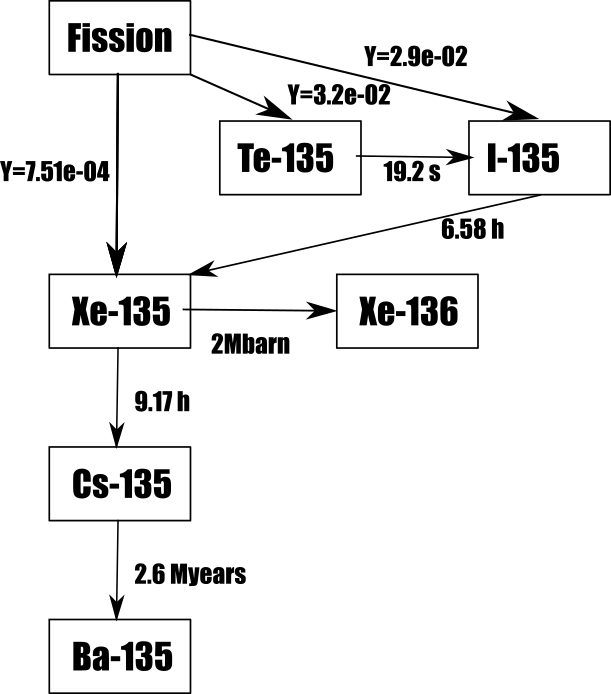
\includegraphics[scale=0.44] {figures/04-xenon.png}}\protect
\caption{\label{fig:xenonprod} \footnotesize{Production of Xenon-135.}}
\end{figure}

We can further simplify the path for Xe-135 since we can notice that Te-135 quickly decays into I-135, thus we can neglect Te-135 altogether and assume that only I-135 is produced from fission. Whereas Xe-135 is produced from fission and from the decay I-135, and it is lost due to its decay with T1/2=9.17h and consumed by absorption. 

Then the system can be expressed with the coupled ODE:


$$ \frac{dN_I}{dt}=Y_I \Sigma_f\varphi-\lambda_I N_I $$

and

$$ \frac{dN_{Xe}}{dt}=Y_{Xe}\Sigma_f\varphi + \lambda_IN_I -\lambda_{Xe}N_{Xe} - \sigma_{Xe}N_{Xe}\varphi  $$

with conditions $N_I(0)=N_{Xe}(0)=0$. (Notice that $\Sigma_f$ depends on the number density of the fissile material, however we can consider that on this time scale it doesn't change with time).

Solving the first equation is rather simple:

$$ N_I(t)=\frac{Y_I\Sigma_f\varphi}{\lambda_I} - \frac{Y_I\Sigma_f\varphi}{\lambda_I}e^{-\lambda_It} $$

\noindent with that the differential equation describing the change of Xenon becomes

$$ \frac{dN_{Xe}}{dt}=Y_{Xe}\Sigma_f\varphi + Y_I\Sigma_f\varphi - Y_I\Sigma_f\varphi e^{-\lambda_It} -\lambda_{Xe}N_{Xe} - \sigma_{Xe}N_{Xe}\varphi  $$

\noindent and the solution becomes

$$ N_{Xe}(t) = c e^{t(-\sigma_{Xe}\varphi - \lambda_{Xe})} + \frac{Y_{Xe}\Sigma_f\varphi}{\sigma_{Xe}\varphi + \lambda_{Xe}} - \frac{Y_I\Sigma_f\varphi}{\sigma_{Xe}\varphi-\lambda_I + \lambda_{Xe}}e^{-\lambda_It} + \frac{Y_{I}\Sigma_f\varphi}{\sigma_{Xe}\varphi + \lambda_{Xe}}  $$

\noindent where 

$$ c= \frac{Y_I\Sigma_f\varphi}{\sigma_{Xe}\varphi-\lambda_I + \lambda_{Xe}}  -\frac{(Y_{I}+Y_{Xe})\Sigma_f\varphi}{\sigma_{Xe}\varphi + \lambda_{Xe}}   $$


The saturation concentrations, when the production and loss terms are in balance ($dN/dt = 0$) are

$$N_I(\infty) = \frac{Y_I\Sigma_f\varphi}{\lambda_I} $$

\noindent and 

$$N_{Xe}(\infty) = \frac{(Y_{Xe}+Y_I)\Sigma_f\varphi}{\lambda_{Xe} + \sigma_{Xe}\varphi} $$

We can observe some things: $\lambda_{Xe}$ is around $10^{-5}$ 1/s, similar order of magnitude as $\sigma_{Xe}\varphi$ if the flux is around $10^{13}$ n/cm-2s (as in a normal reactor).  Notice, that for low ($\leq$ $10^{12}$) fluxes (eg. a training reactor)  the $\sigma_{Xe}\varphi$ can be neglected (since it is much smaller than $\lambda_{Xe}$, and the saturation concentration is proportional to the flux. If the flux is high ($\geq$ $10^{14}$) (eg. in a research reactor), the $\lambda_{Xe}$ can be neglected (since it is much smaller than $\sigma_{Xe}\varphi$, and then the saturation concentration is independent from the flux. In reality the flux is usually somewhere in between, the concentration is not proportional anymore to the flux, but still grows with it.


Let's see what happens after the concentrations saturated and we shutdown the reactor. The ODEs simplify to (note, flux is zero)

$$ \frac{dN_I}{dt}=-\lambda_IN_I $$

\noindent and

$$ \frac{dN_{Xe}}{dt}= \lambda_IN_I -\lambda_{Xe}N_{Xe} $$

\noindent with conditions $N_I(0)=N_I(\infty)$ $N_{Xe}(0)=N_{Xe}(\infty)$

\noindent where the notation might be a bit confusing, nevertheless the infinite values refers to the previously obtained functions.

Then

$$ N_I(t)=N_I(\infty)e^{-\lambda_It} $$

$$ N_{Xe}(t) = c e^{-\lambda_{Xe}t} - \frac{\lambda_I}{\lambda_I - \lambda_{Xe}}N_I(\infty)e^{-\lambda_{I}t} $$

\noindent where

$$ c = N_{Xe}(\infty)+\frac{\lambda_I}{\lambda_I - \lambda_{Xe}}N_I(\infty) $$

\noindent thus

%$$ N_{Xe} (t) = N_{Xe}(\infty)e^{-\lambda_{Xe}t}+\frac{\lambda_I}{\lambda_I - \lambda_{Xe}}N_I(\infty)e^{-\lambda_{Xe}t} - \frac{\lambda_I}{\lambda_I - \lambda_{Xe}}N_I(\infty)e^{-\lambda_{I}t} $$

$$ N_{Xe} (t) = N_{Xe}(\infty)e^{-\lambda_{Xe}t}+\frac{\lambda_I}{\lambda_I - \lambda_{Xe}}N_I(\infty)(e^{-\lambda_{Xe}t} - e^{-\lambda_{I}t}) $$

The left side of Figure \ref{fig:xenonpois} shows the change in the Xenon concentration after shutdown. First, the concentration increases: no Xe is lost anymore due to absorption, and since the half life of I-135 is shorter, it builds more Xe-135 than what the decay of Xe-135 removes. After couple of hours, a large part of I-135 is lost, thus the decay of Xe-135 dominates, and the Xe concentration starts to drop. Depending on flux, it might take more than a day to reach the same Xe concentration as right after shutdown. Sometimes, the amount of Xe is quantified with the \textit{Xenon-poisoning factor}: $\Sigma_{a,Xe}/\Sigma_{a,U}$, which shows a similar trend in the right side of Figure \ref{fig:xenonpois}, but the numeric values are more practical.

\begin{figure}[ht!]
\protect \centering{
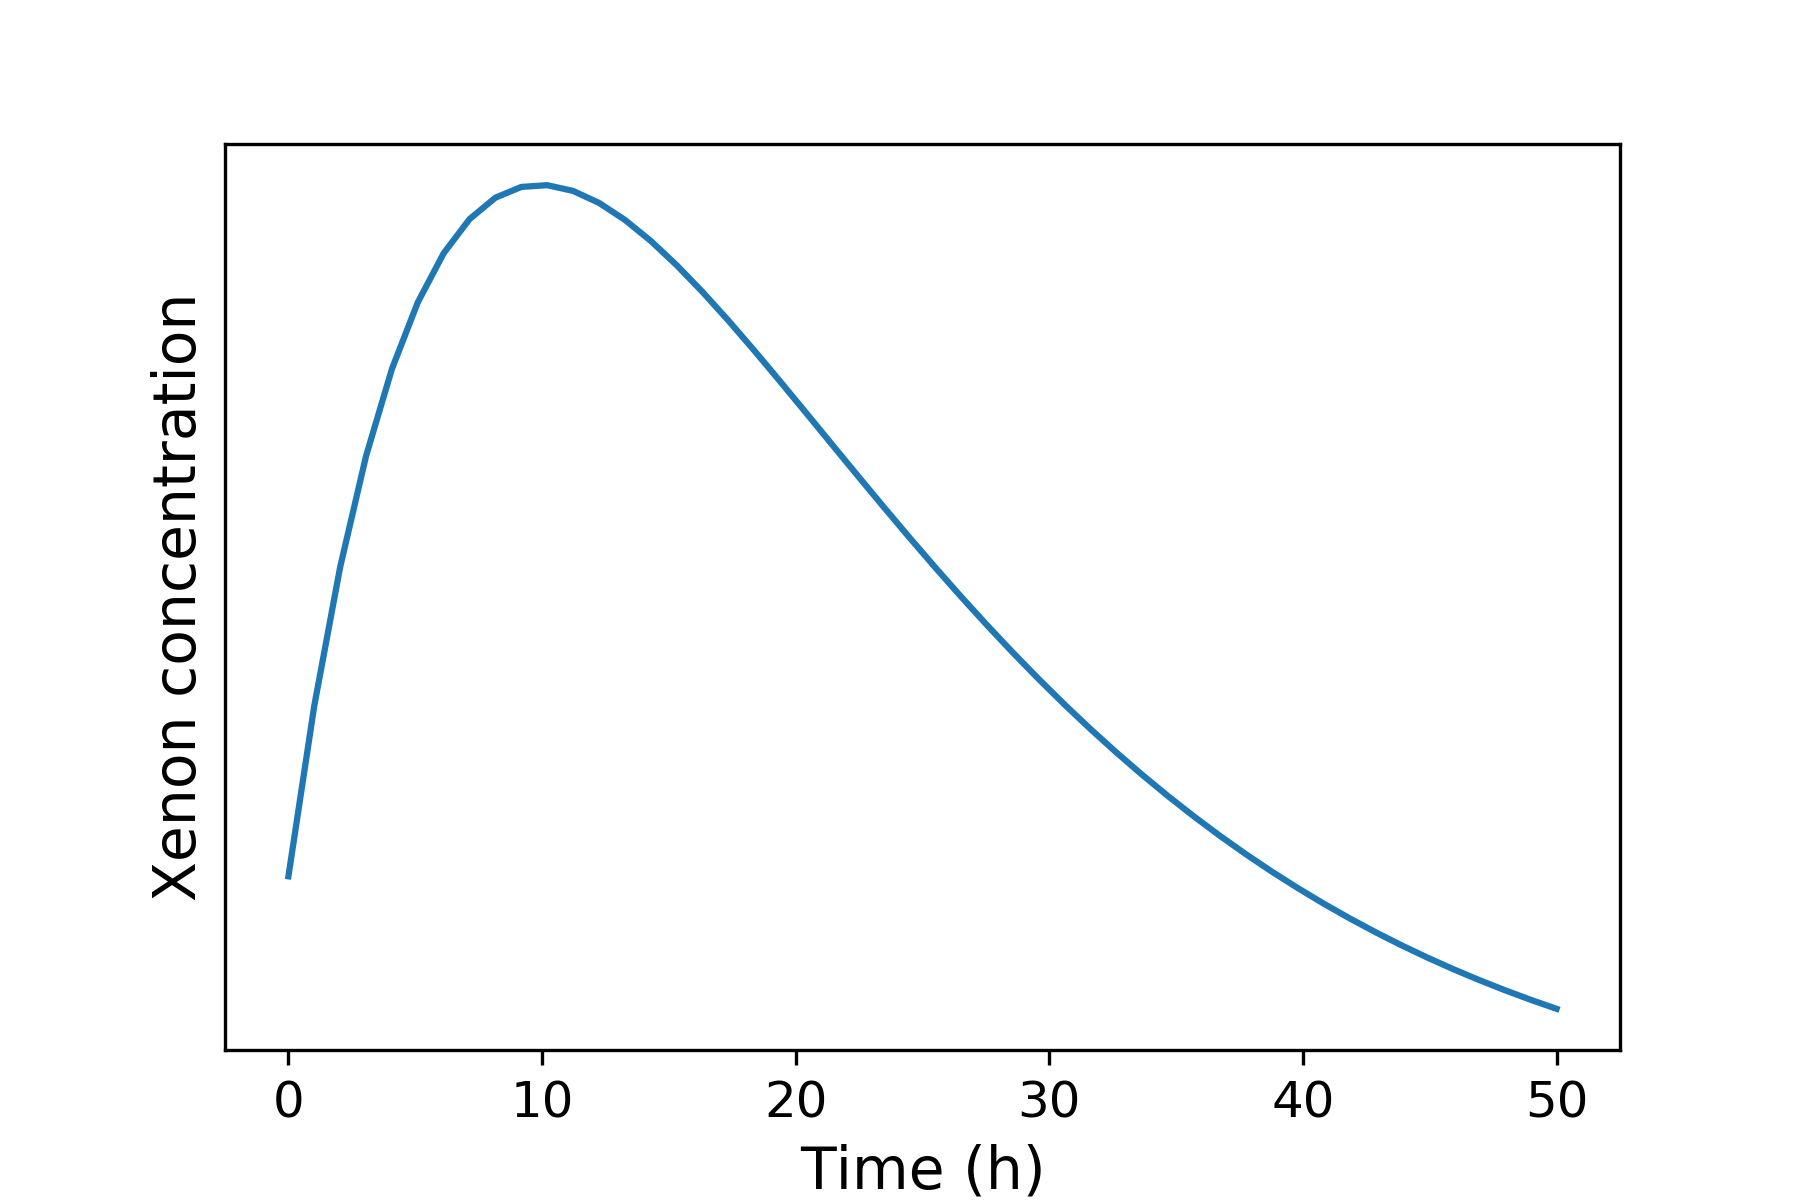
\includegraphics[scale=0.43] {figures/04-xenonconcentration.png}
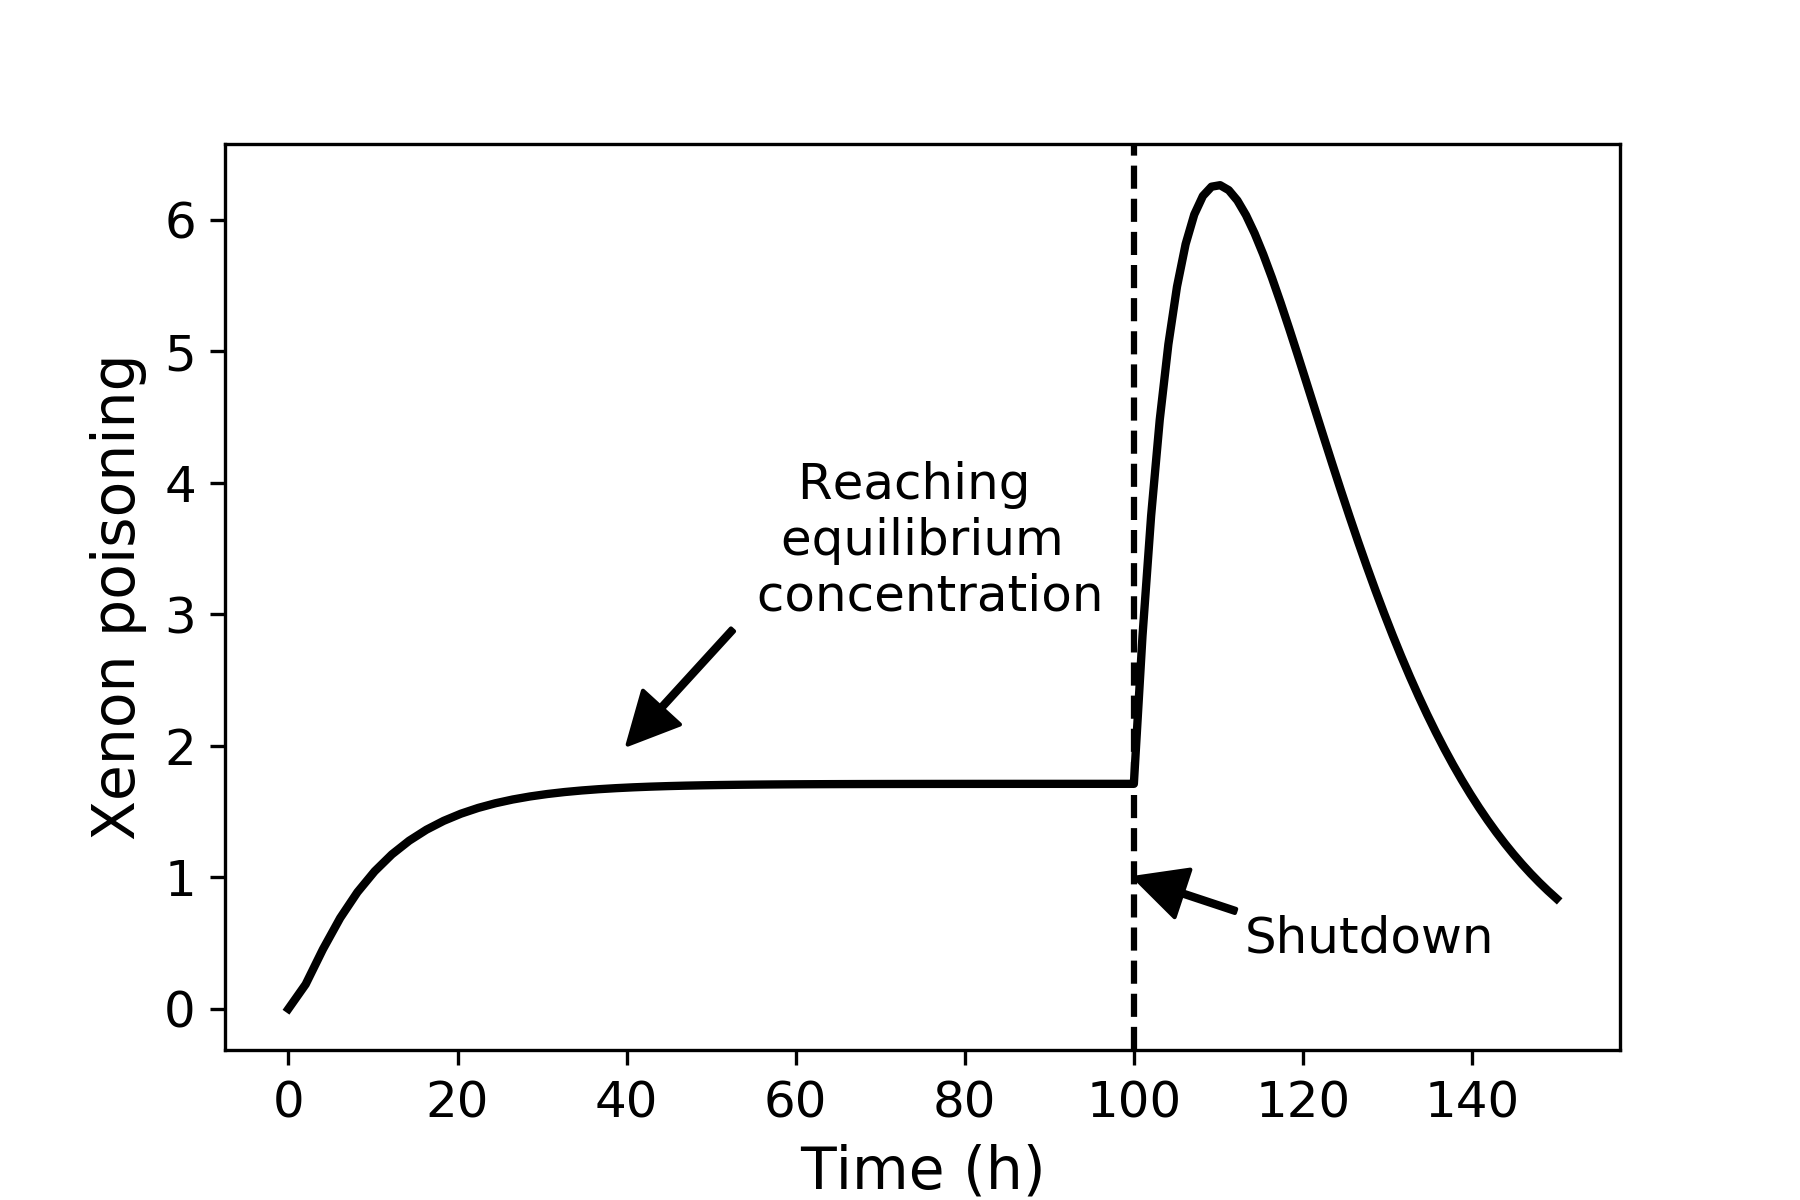
\includegraphics[scale=0.43] {figures/04-xenonpoisoning.png}}\protect
\caption{\label{fig:xenonpois} \footnotesize{Change of Xenon-135 concentration after shutdown and xenon poisoning during operation..}}
\end{figure}

Due to Xenon-poisoning, the reactivity of the core decreases after shutdown. Thus, if the operators are not able to pull out enough control rods, it might not be possible to restart the reactor safely. This was partly the cause beind the Chernobyl accident\footnote{For further details \url{https://nuclidecalendar.github.io/days/dec13.html}}. One has to also mention that Xe-poisoning might have strong spatial effects. 

\subsubsection{Burnable absorbers}

Some times introducing a reactor poison into the core is intentional. This is the case when burnable absorbers (for example boron or gadolinium) are mixed to the fuel. While the excess positive reactivity of the fuel is depleted, the negative reactivity of the burnable absorbers is decreasing. However, since burnable absorbers are usually only introduces in some of the fuel rods, their use may lead to non-uniform neutron flux distribution.

%\end{document}